\section{METODOLOGÍA}
En el presente capítulo se muestra el procedimiento que se desarrollo para la elaboración de la metodología que se propone, basado en las actividades previas y la descripción de los pasos a seguir, manipulando y monitoreando la informacíon de sensores y actuadores mediante el dispositivo móvil.

\subsection{ESTRUCTURA GENERAL}

Se presenta una estructura general de comunicación donde se incluye un bosquejo del flujo de la comunicación entre los actuadores y sensores utilizados hasta el dispositivo móvil. esta propuesta se divide en 5 fases principales: i) Aplicación móvil, ii) Conectividad, iii) Tarjeta electrónica, iv) Circuito de potencia y v) Actuadores y sensores.

%
\begin{figure}[H]
%\vspace{0.2cm}
\centering
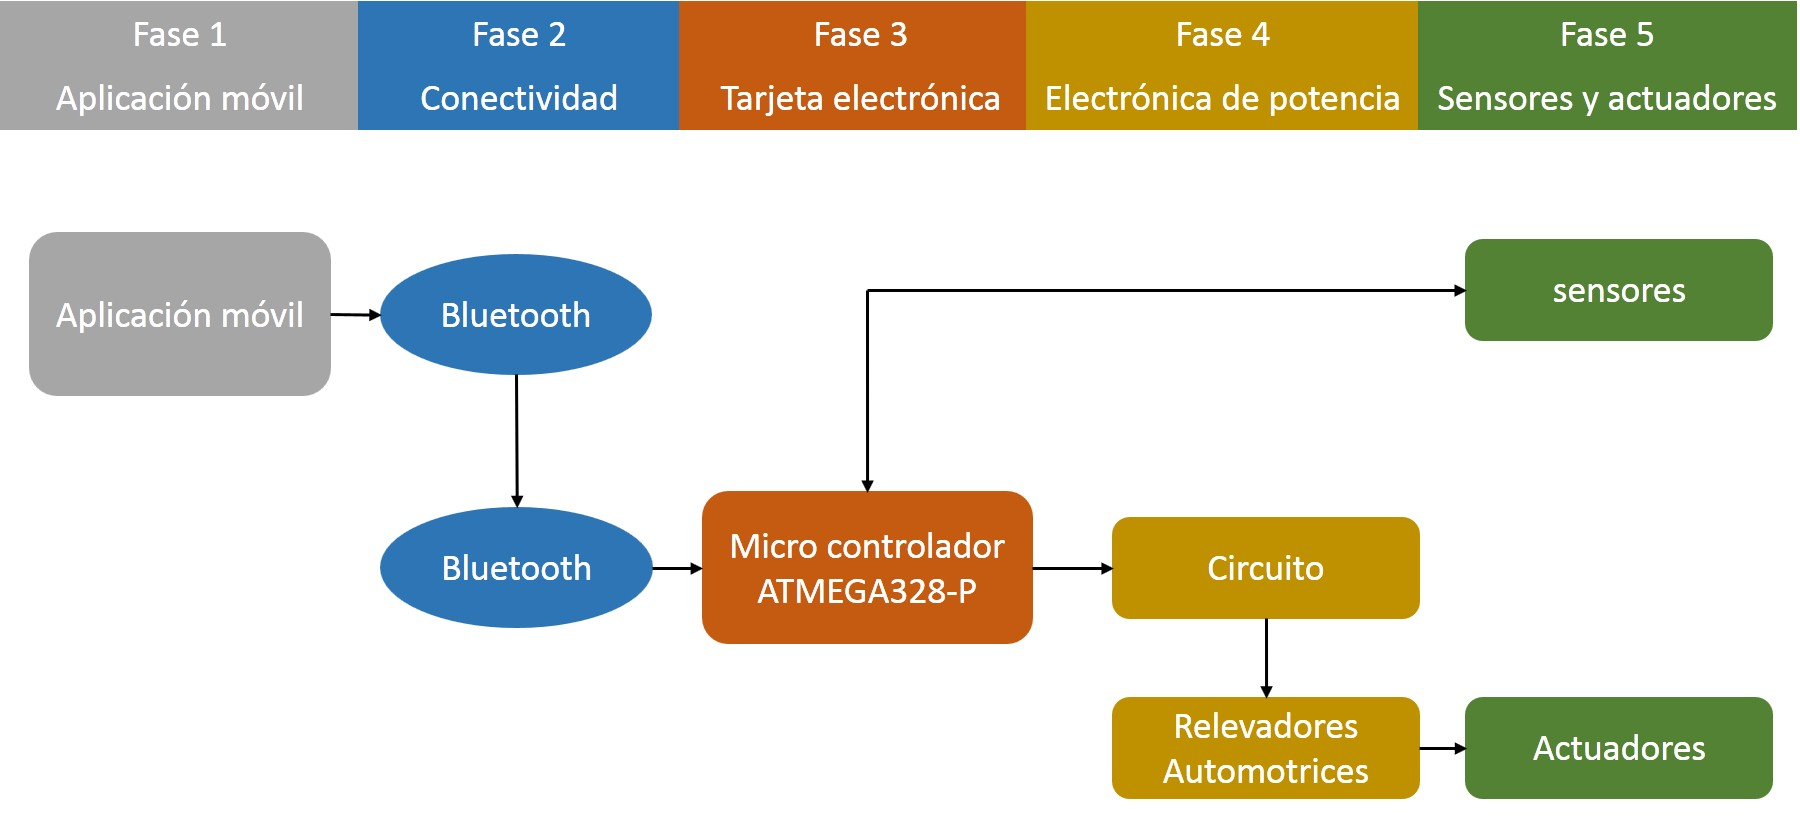
\includegraphics[width=0.95\textwidth]{metodologia/fig_1.jpg}
\caption{Estructura general de comunicación}
\label{Meuno}
\end{figure}
%

 
 Tal como se muestra en la Figura \ref{Meuno} el proceso de manipulación y monitoreo se describe en la siguiente lista.
 \begin{enumerate}
\item La aplicación móvil se inicia y envia comandos.
\item Los comandos son enviados a través de la comunicación inalámbrica Bluetooth.
\item La placa electrónica recibe los datos por medio del Bluetooth y regresa una repuesta.
\item Según los datos activa o desactiva ciertas señales que encienden o apagan un relevador por medio del circuito de potencia.
\item El relevador transmite o evita el paso de la señal \textit{Low} hacia el actuador.
\item El actuador se activa o desactiva segun la transmisión del relevador.

\end{enumerate}


\subsection{APLICACION MÓVIL}

La aplicación móvil se desarrolló por medio de la plataforma Android Studio\textregistered enfocada al sistema operativo Android, los requisitos mínimos de \textit{software} para que el paquete de aplicaciones Android (APK del inglés \textit{Android Application Package}) funcione de manera correcta es necesario tener una versión mínima de Android 3.0. La estructura general de la aplicación móvil se muestra en la Figura \ref{Mestrucgeral}.\\

%
\begin{figure}[H]
%\vspace{0.2cm}
\centering
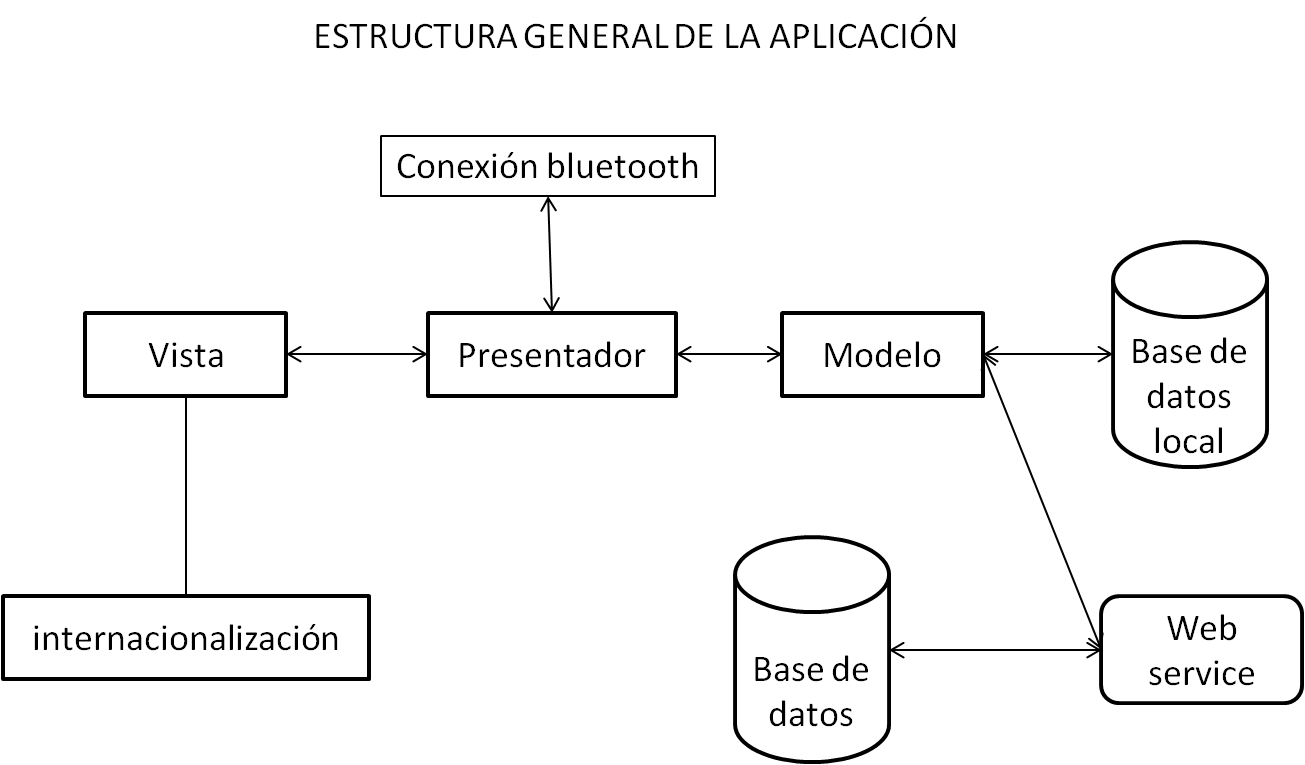
\includegraphics[width=0.95\textwidth]{metodologia/fig1.png}
\caption{Estructura general de la aplicación.}
\label{Mestrucgeral}
\end{figure}
%


La aplicación se desarrollo siguiendo un patrón de arquitectura Modelo-Vista-Presentador, debido a la relación de diseño, actividad y datos, usado comunmente en la construcción de interfaces de usuario. Este patrón permite una escalabilidad sencilla y una estructura independiente para cada capa, permitiendo realizar modificaciones de una forma muy fácil a la capa seleccionada.\\

La capa de presentación esta programada para actuar como intermediario entre la vista y el modelo.  Se encarga de tomar acciones mediante las reglas de negocio cuando el usuario interactua con la vista y recupera los datos del modelo enviandolos en formato necesario para la vista. En la capa vista se diseño toda la interfaz para el usuario y su unica funcionalidad es llamar a un método de la capa presentación cada vez que hay una acción en la interfaz. Y finalmente en la capa de modelo se recuperan los datos y se hace la conexión con un servicio Web y una base de datos donde se consulta la información mediante procedimientos almacenados.\\

La aplicación cuenta con la internacionalización, una práctica de diseño y desarrollo que facilita la migración del contenido en el futuro, ya que eliminar obstáculos a la localización o la distribución internacional. Permitiendo modificar el idioma de la vista de manera sencilla al almacenar todos los textos en variables y ubicarlos en un solo archivo.\\

Se diseño el diagrama de clases de la aplicación móvil tal cual se muestra en la Figura \ref{diaclas}, existen 5 clases de entidades en el diagrama. 
%
\begin{figure}[H]
%\vspace{0.2cm}
\centering
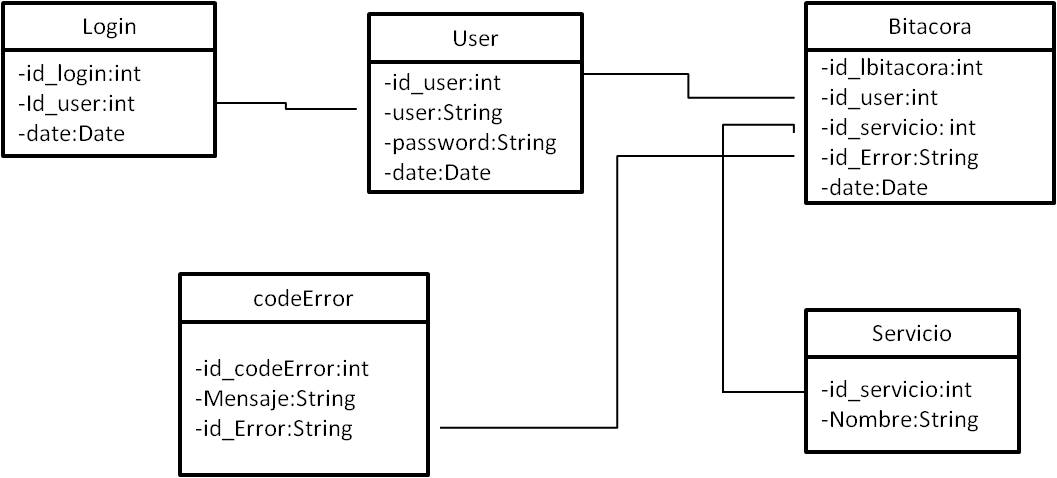
\includegraphics[width=0.95\textwidth]{metodologia/DClases.jpg}
\caption{Diagrama de clases de la aplicación móvil.}
\label{diaclas}
\end{figure}
%
\begin{enumerate}
\item  clase \textit{Login}: esta entidad representa el historial de acceso a la aplicación, el usuario cada vez que accede la aplicación se registra en la base de datos. Los atributos incluidos de la clase \textit{login} son idlogin, iduser, date.
\item clase \textit{User}: esta entidad representa el acceso a la aplicación, cada vez que el usuario accede se tiene que revisar la base de datos con la información ingresada. Los atributos includos de la clase \textit{User} son iduser, user, password, date.
\item clase \textit{codeError}: esta entidad representa los codigos de posibles errores, cuando existe un error se muestra un mensaje en la aplicación sobre el error en la base de datos al guardar o extraer algún dato. Los atributos incluidos de la clase \textit{codeError} son idcode, Mensaje, iderror.
\item clase \textit{service}: esta entidad representa los servicios que se pueden realizar por ejemplo encender el vehículo, subir los vidrios, entre otros.Esta información se utiliza para guardar el historial de servicios. Los atributos incluidos de la clase \textit{service} son idservicio, nombre.
\item clase \textit{bitacora}: esta entidad representa el historial de servicios que se han realizado en la aplicación. Los atributos incluidos de la clase \textit{bitacora} son idbitacora, iduser, idservice, iderror, date.
\end{enumerate}
Los diagramas de secuencia describen el funcionamiento del proceso y como se ha pasado el mensaje en una secuencia temporal, la información se envia a través de parametros mediante un objecto de transferencia de datos, cuya responsabilidad es almacenar y entregar sus propios datos entre las diferentes capas. La Figura \ref{ds1} describe la secuencia de eventos para iniciar sesión.

%
\begin{figure}[H]
%\vspace{0.2cm}
\centering
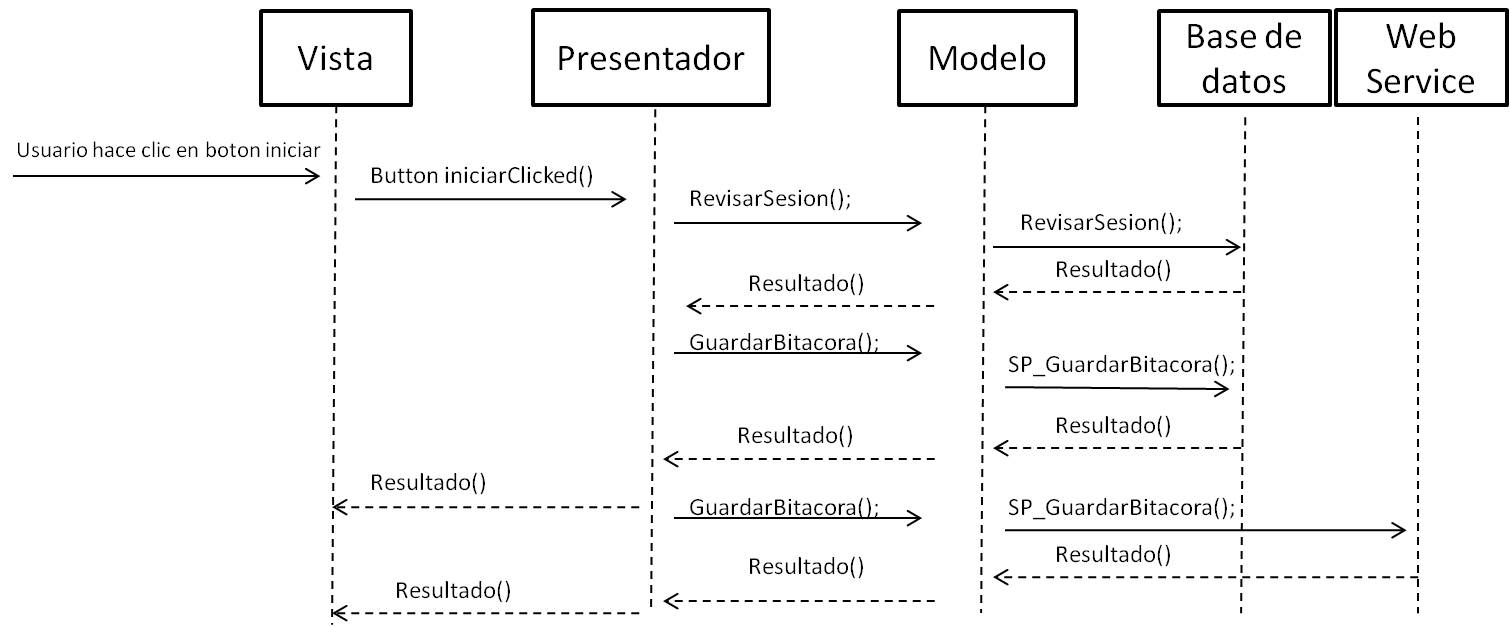
\includegraphics[width=0.95\textwidth]{metodologia/DSIniciarSesion.jpg}
\caption{Diagrama de secuencia del flujo de inicio de sesión.}
\label{ds1}
\end{figure}
%

 \begin{enumerate}
\item El usuario inicia la aplicación, inserta su usuario y su contraseña después al oprimir el boton iniciar se pasa a la capa de presentador.
\item La capa de presentador toma los datos del usuario y la contraseña y los envia a través de la capa modelo hacia la base de datos local, verificando que coincidan los datos.
\item La base de datos regresa una respuesta a la capa de modelo y regresa el resultado a la capa presentador.
\item La capa presentador revisa el resultado según las reglas de negocio establecidas y dependiendo del dato cambia la vista o manda un mensaje de error.
\item La capa presentador envia una petición de guardado hacia la base de datos para el registro de las actividades en la aplicación formando un historial, al igual que envia la información de la bitacora hacia el servicio web para crear un registro de la aplicación en linea.
\end{enumerate}

La Figura \ref{ds2} se muestra el evento de la secuencia del inicio del Bluetooth
%
\begin{figure}[H]
%\vspace{0.2cm}
\centering
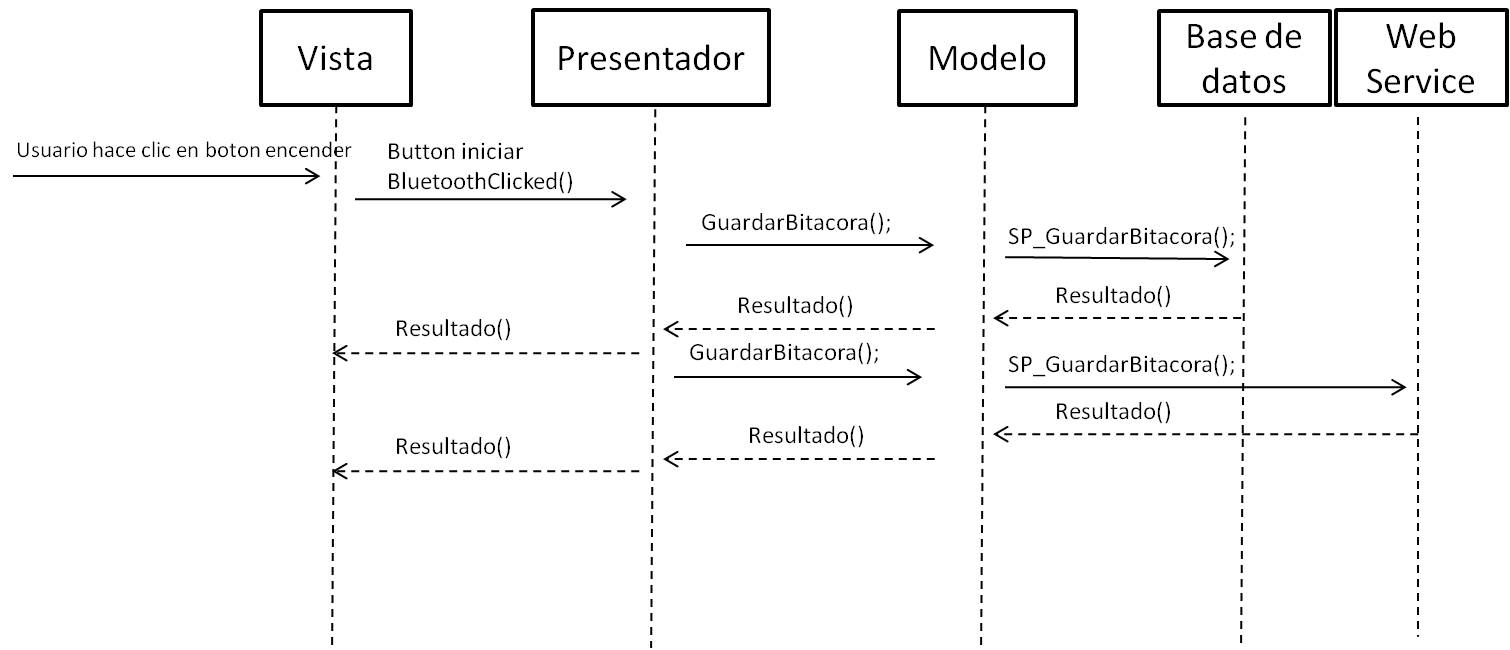
\includegraphics[width=0.95\textwidth]{metodologia/DSIniciarBluetooth.jpg}
\caption{Diagrama de secuencia del flujo de inicio del Bluetooth.}
\label{ds2}
\end{figure}


 \begin{enumerate}
\item El usuario preciona el boton para activar la conexión del Bluetooth.
\item La capa de presentador ejecuta la acción de encender la señal del Bluetooth.
\item{La capa presentador envia a la capa vista la información necesaria para cambiar de pantalla o enviar un mensaje de error}.
\item La capa presentador envia una petición de guardado hacia la base de datos para el registro de las actividades en la aplicación formando un historial, al igual que envia la información de la bitacora hacia el servicio web para crear un registro de la aplicación en linea.
\end{enumerate}

La Figura \ref{ds3} se muestra el evento de la secuencia del menu de opciones de la aplicación.
%
\begin{figure}[H]
%\vspace{0.2cm}
\centering
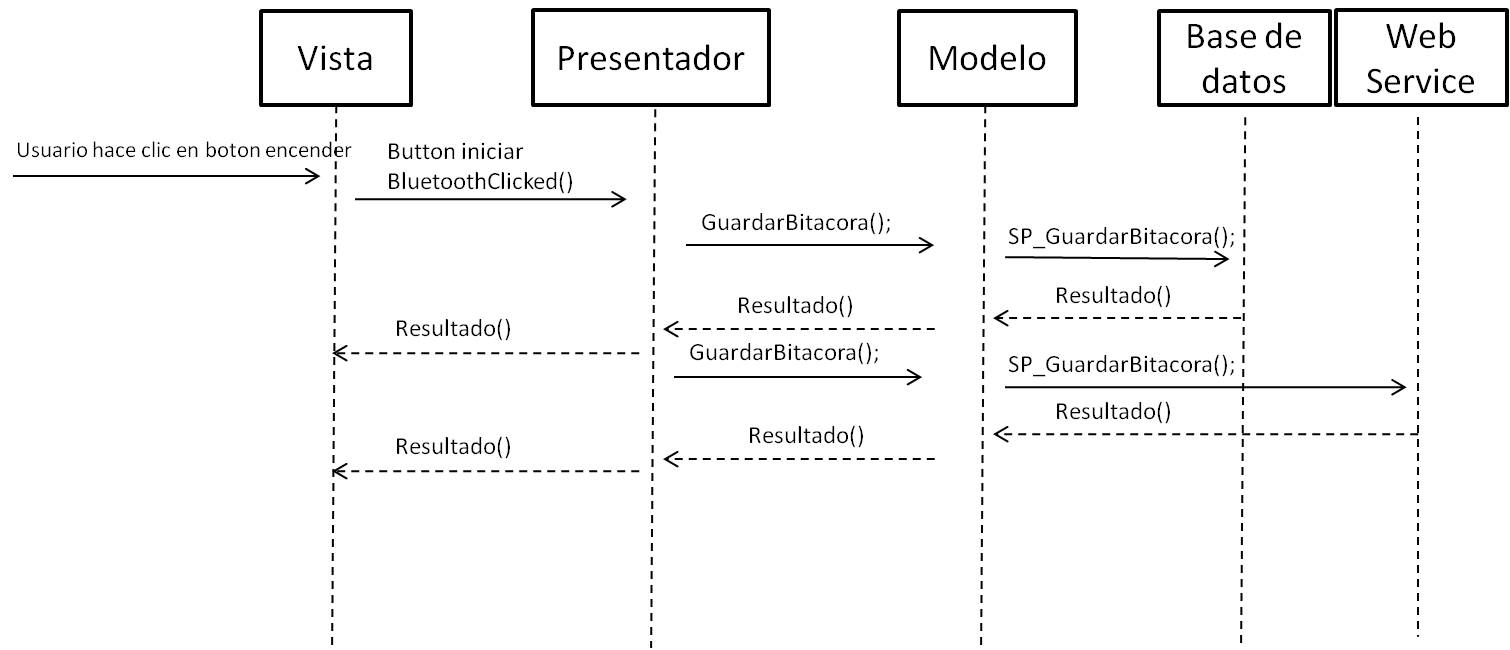
\includegraphics[width=0.95\textwidth]{metodologia/DSIniciarBluetooth.jpg}
\caption{Diagrama de secuencia del flujo del menu de opciones de la aplicación.}
\label{ds3}
\end{figure}
%

 \begin{enumerate}
\item El usuario selecciona una opción del menu.
\item La capa de presentador toma la información de la opción seleccionada y regresa a la vista la nueva pantalla o un mensaje de error.
\item La capa presentador envia una petición de guardado hacia la base de datos para el registro de las actividades en la aplicación formando un historial, al igual que envia la información de la bitacora hacia el servicio web para crear un registro de la aplicación en linea.
\end{enumerate}

La Figura \ref{ds4} se muestra el evento de la secuencia de subir el vidrio.\\
\begin{figure}[H]
%\vspace{0.2cm}
\centering
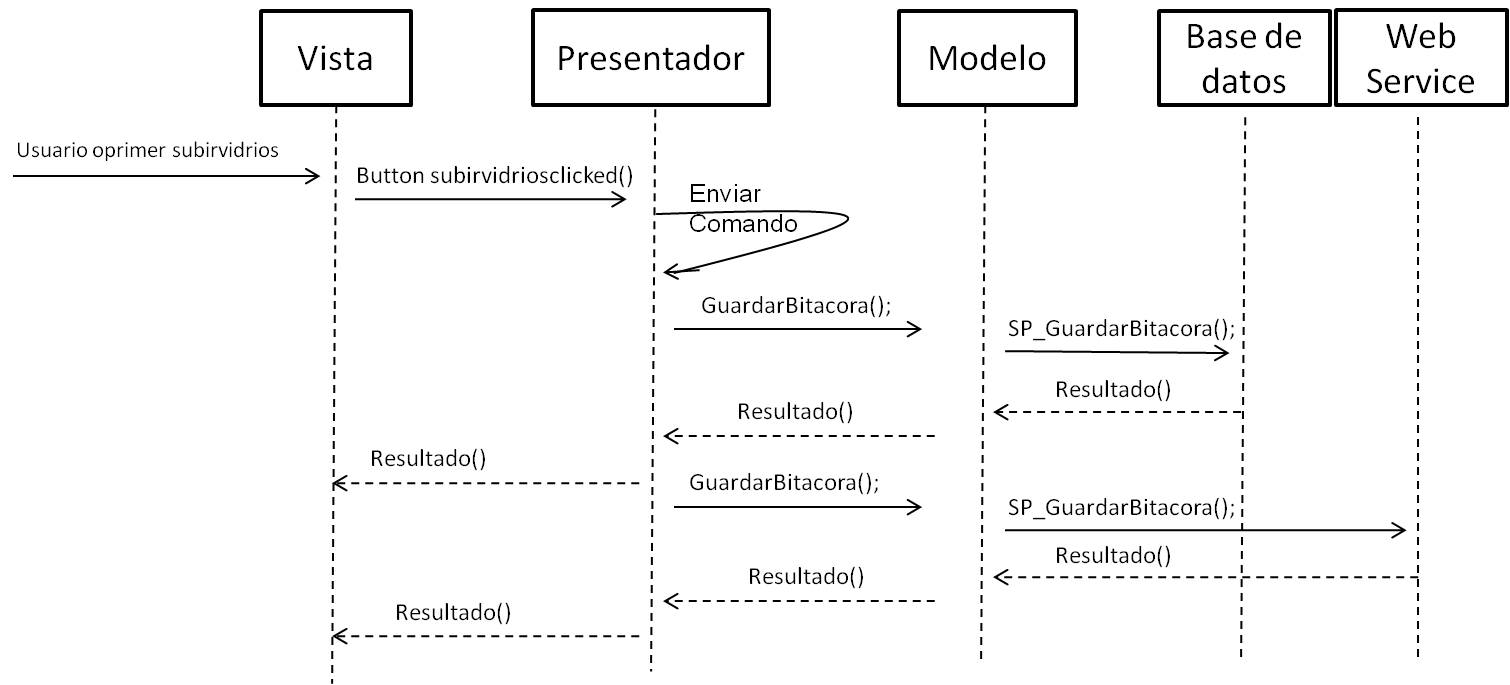
\includegraphics[width=0.95\textwidth]{metodologia/DSSubirVidrios.jpg}
\caption{Diagrama de secuencia del flujo de la funcionalidad subir vidrios.}
\label{ds4}
\end{figure}
%
 \begin{enumerate}
\item El usuario selecciona la opción de subir vidrios.
\item La capa de presentador toma la información de la opción seleccionada y la envia via Bluetooth a la tarjeta electrónica y espera una respuesta de la tarjeta electrónica por el mismo medio de comunicación.
\item Después de adquirir la respuesta envia a la pantalla un mensaje.
\item La capa presentador envia una petición de guardado hacia la base de datos para el registro de las actividades en la aplicación formando un historial, al igual que envia la información de la bitacora hacia el servicio web para crear un registro de la aplicación en linea.
\end{enumerate}

La Figura \ref{ds5} se muestra el evento de la secuencia de bajar el vidrio.\\
\begin{figure}[H]
%\vspace{0.2cm}
\centering
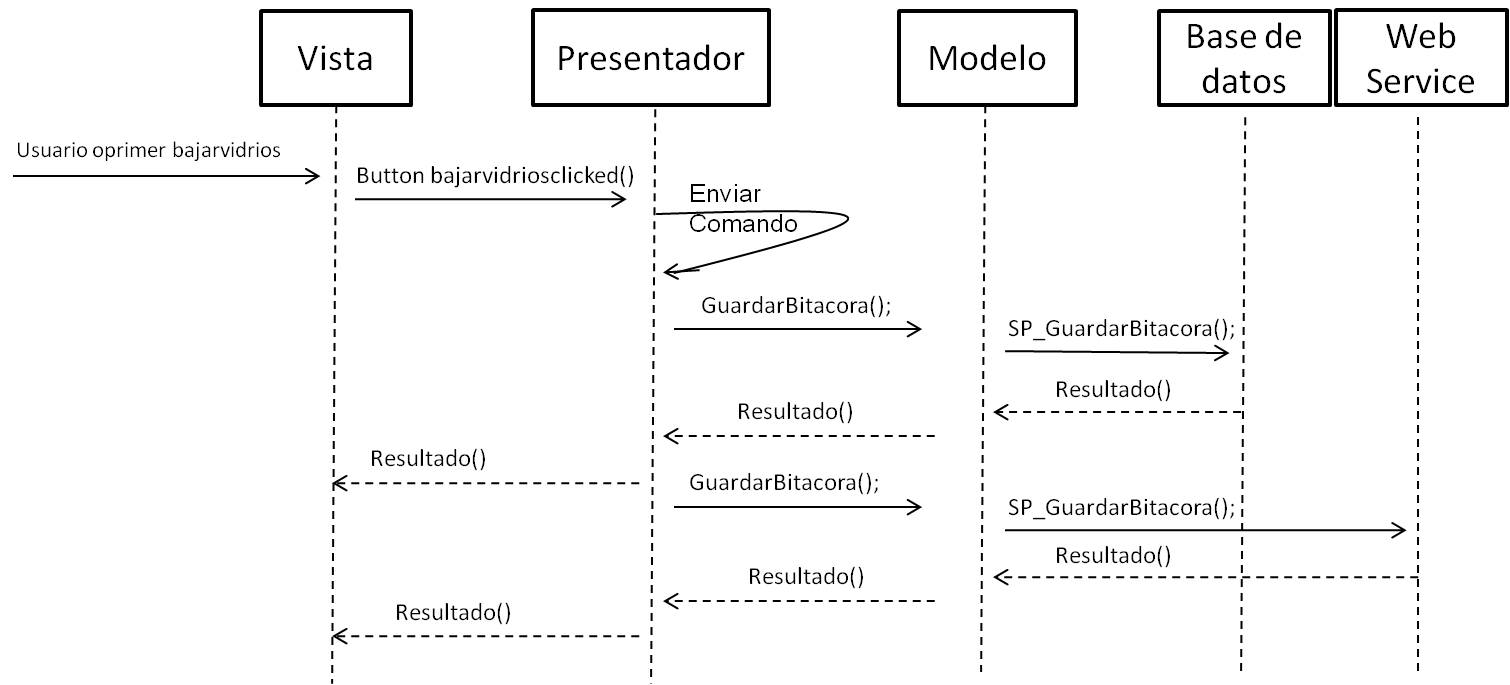
\includegraphics[width=0.95\textwidth]{metodologia/DSbajarvidrios.jpg}
\caption{Diagrama de secuencia del flujode la funcionalidad bajar vidrios.}
\label{ds5}
\end{figure}
%
 \begin{enumerate}
\item El usuario selecciona la opción de bajar vidrios.
\item La capa de presentador toma la información de la opción seleccionada y la envia via Bluetooth a la tarjeta electrónica y espera una respuesta de la tarjeta electrónica por el mismo medio de comunicación.
\item Después de adquirir la respuesta envia a la pantalla un mensaje.
\item La capa presentador envia una petición de guardado hacia la base de datos para el registro de las actividades en la aplicación formando un historial, al igual que envia la información de la bitacora hacia el servicio web para crear un registro de la aplicación en linea.
\end{enumerate}

La Figura \ref{ds6} se muestra el evento de la secuencia de poner seguro a las puertas.\\
\begin{figure}[H]
%\vspace{0.2cm}
\centering
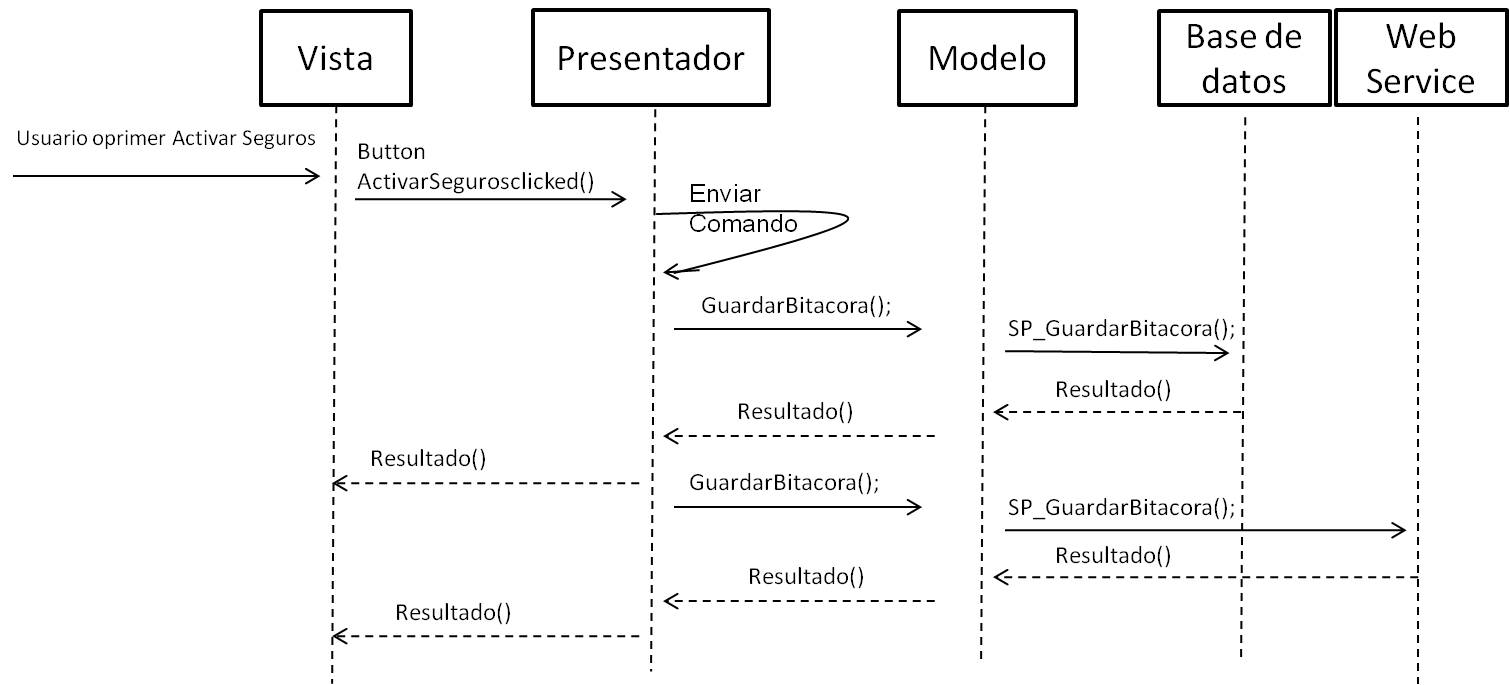
\includegraphics[width=0.95\textwidth]{metodologia/DSActivarSeguros.jpg}
\caption{Diagrama de secuencia del flujo de la funcionalidad activar seguros.}
\label{ds6}
\end{figure}
%
 \begin{enumerate}
\item El usuario selecciona la opción de poner seguro en las puertas.
\item La capa de presentador toma la información de la opción seleccionada y la envia via Bluetooth a la tarjeta electrónica y espera una respuesta de la tarjeta electrónica por el mismo medio de comunicación.
\item Después de adquirir la respuesta envia a la pantalla un mensaje.
\item La capa presentador envia una petición de guardado hacia la base de datos para el registro de las actividades en la aplicación formando un historial, al igual que envia la información de la bitacora hacia el servicio web para crear un registro de la aplicación en linea.
\end{enumerate}

La Figura \ref{ds7} se muestra el evento de la secuencia de quitar el seguro de las puertas.\\
\begin{figure}[H]
%\vspace{0.2cm}
\centering
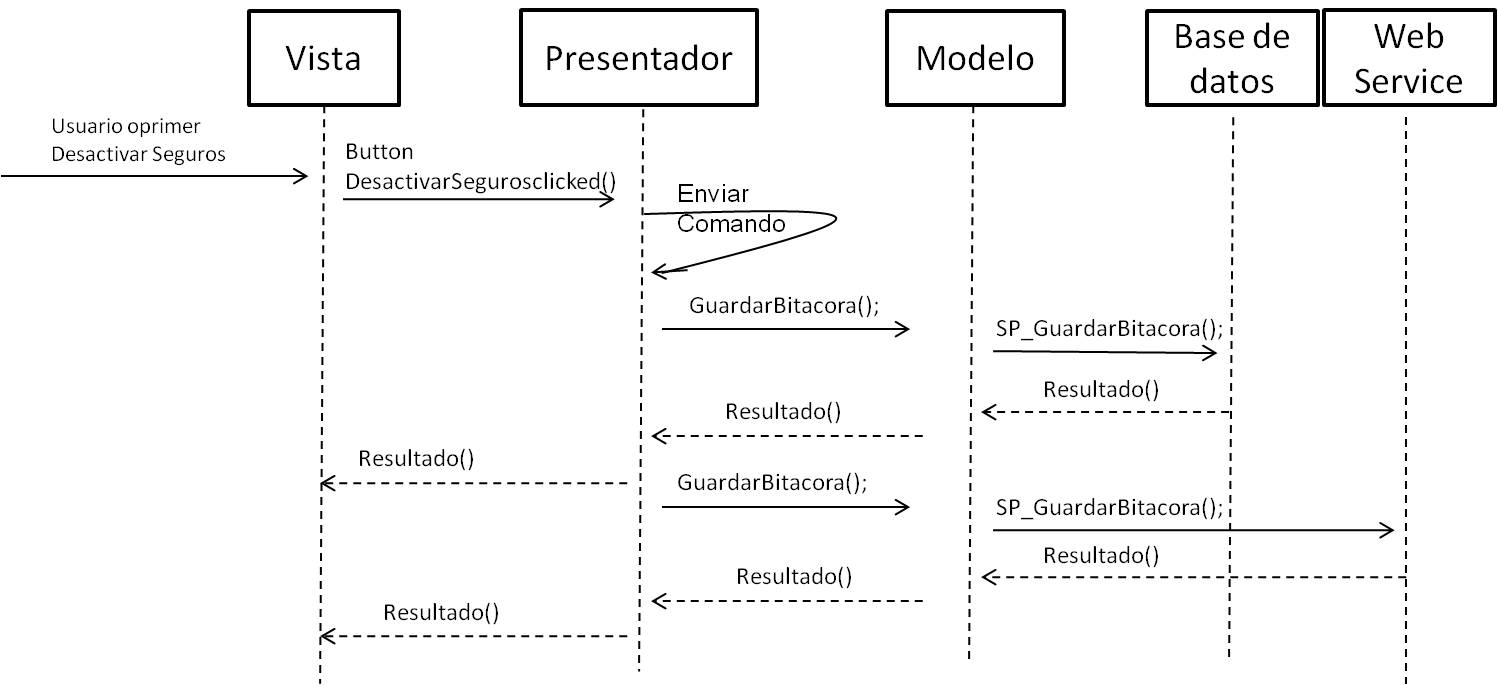
\includegraphics[width=0.95\textwidth]{metodologia/DSDesactivarSeguros.jpg}
\caption{Diagrama de secuencia del flujo de la funcionalidad desactivar seguros.}
\label{ds7}
\end{figure}
%
 \begin{enumerate}
\item El usuario selecciona la opción de quitar seguro en las puertas.
\item La capa de presentador toma la información de la opción seleccionada y la envia via Bluetooth a la tarjeta electrónica y espera una respuesta de la tarjeta electrónica por el mismo medio de comunicación.
\item Después de adquirir la respuesta envia a la pantalla un mensaje.
\item La capa presentador envia una petición de guardado hacia la base de datos para el registro de las actividades en la aplicación formando un historial, al igual que envia la información de la bitacora hacia el servicio web para crear un registro de la aplicación en linea.
\end{enumerate}

La Figura \ref{ds8} se muestra el evento de la secuencia de activar o desactivar las luces interiores.\\
\begin{figure}[H]
%\vspace{0.2cm}
\centering
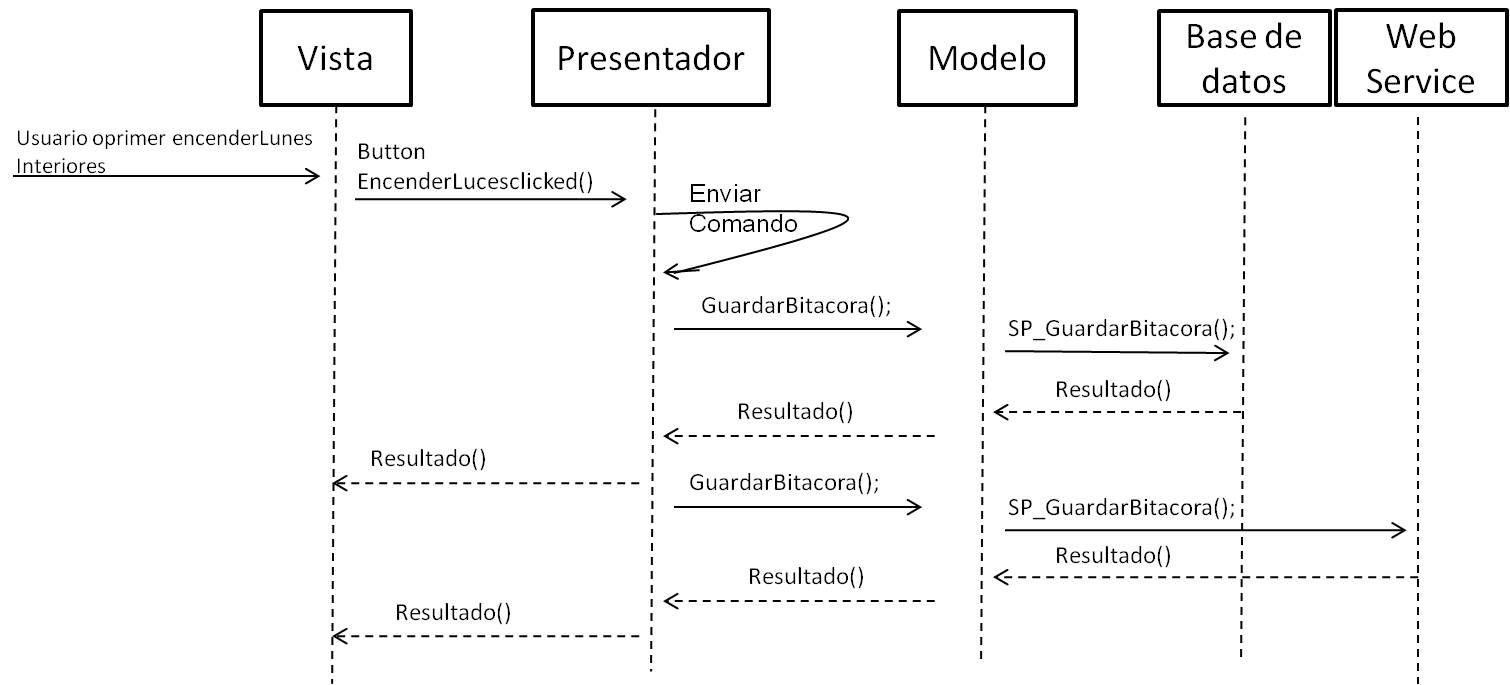
\includegraphics[width=0.95\textwidth]{metodologia/DSEncenderLucesInteriores.jpg}
\caption{Diagrama de secuencia del flujode la funcionalidad encender/apgar luces interiores.}
\label{ds8}
\end{figure}
%
 \begin{enumerate}
\item El usuario selecciona la opción de luces interiores.
\item La capa de presentador toma la información de la opción seleccionada y la envia via Bluetooth a la tarjeta electrónica y espera una respuesta de la tarjeta electrónica por el mismo medio de comunicación.
\item Después de adquirir la respuesta envia a la pantalla un mensaje.
\item La capa presentador envia una petición de guardado hacia la base de datos para el registro de las actividades en la aplicación formando un historial, al igual que envia la información de la bitacora hacia el servicio web para crear un registro de la aplicación en linea.
\end{enumerate}

La Figura \ref{ds9} se muestra el evento de la secuencia de activar o desactivar las luces exteriores.\\
\begin{figure}[H]
%\vspace{0.2cm}
\centering
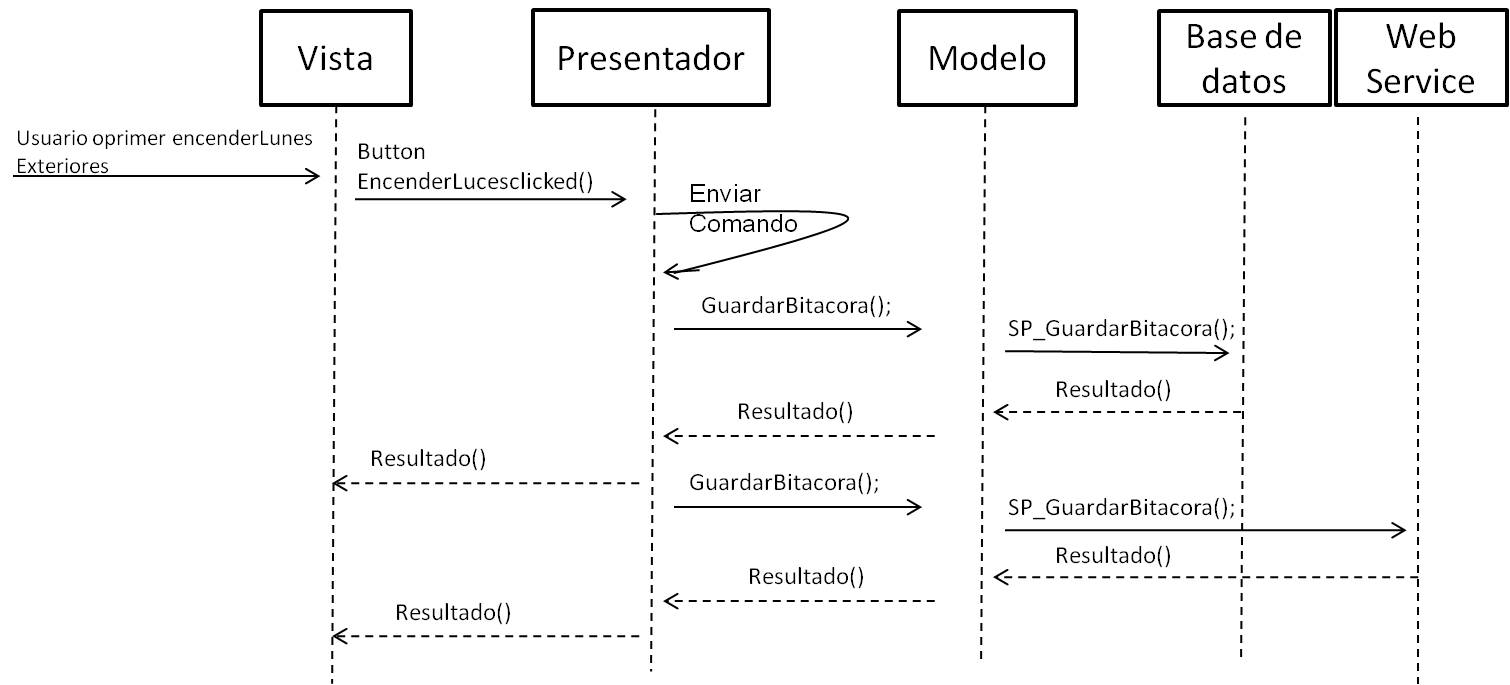
\includegraphics[width=0.95\textwidth]{metodologia/DSEncenderLucesExteriores.jpg}
\caption{Diagrama de secuencia del flujo de la funcionalidad encender/apagar luces exteriores.}
\label{ds9}
\end{figure}
%
 \begin{enumerate}
\item El usuario selecciona la opción de luces exteriores.
\item La capa de presentador toma la información de la opción seleccionada y la envia via Bluetooth a la tarjeta electrónica y espera una respuesta de la tarjeta electrónica por el mismo medio de comunicación.
\item Después de adquirir la respuesta envia a la pantalla un mensaje.
\item La capa presentador envia una petición de guardado hacia la base de datos para el registro de las actividades en la aplicación formando un historial, al igual que envia la información de la bitacora hacia el servicio web para crear un registro de la aplicación en linea.
\end{enumerate}



La Figura \ref{ds10} se muestra el evento de la secuencia de abrir la cajuela.\\
\begin{figure}[H]
%\vspace{0.2cm}
\centering
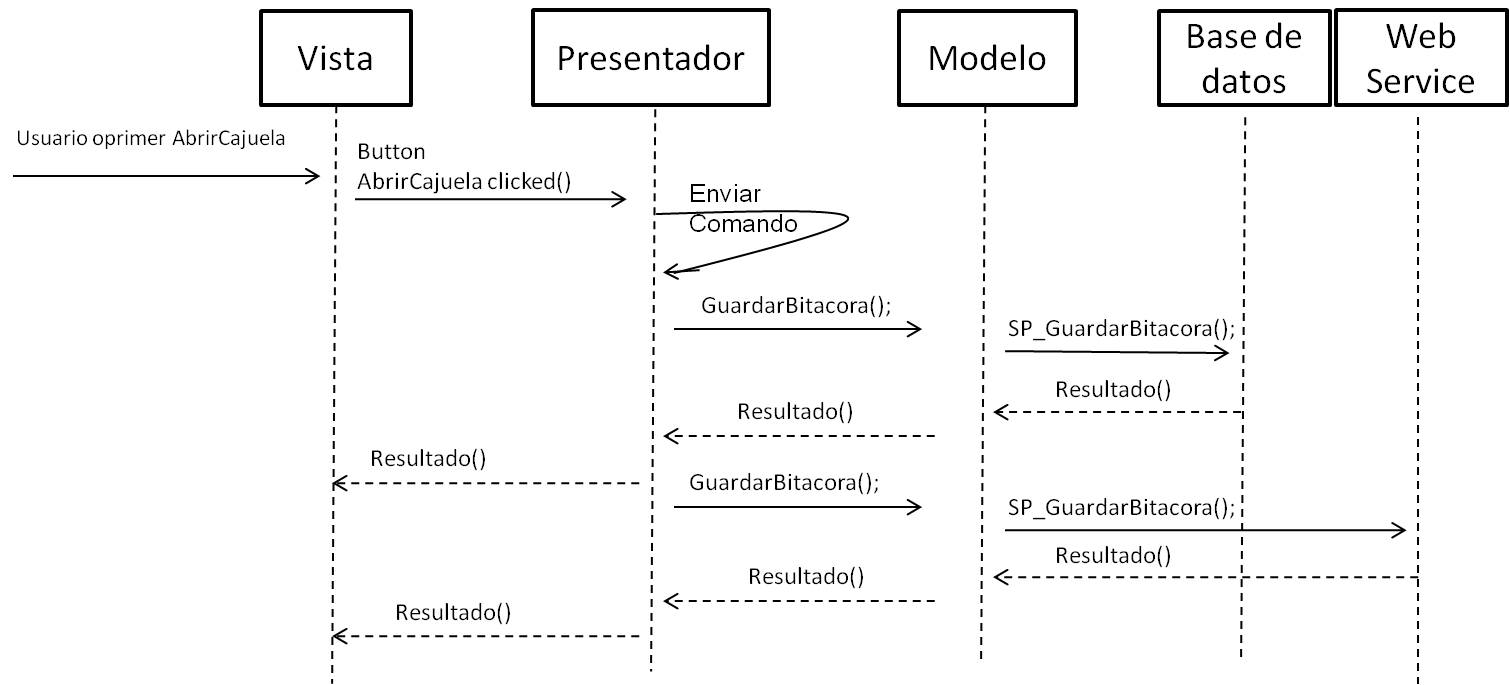
\includegraphics[width=0.95\textwidth]{metodologia/DSAbrirCajuela.jpg}
\caption{Diagrama de secuencia del flujo de la funcionalidad abrir cajuela.}
\label{ds10}
\end{figure}
%
 \begin{enumerate}
\item El usuario selecciona la opción de abrir cajuela.
\item La capa de presentador toma la información de la opción seleccionada y la envia via Bluetooth a la tarjeta electrónica y espera una respuesta de la tarjeta electrónica por el mismo medio de comunicación.
\item Después de adquirir la respuesta envia a la pantalla un mensaje.
\item La capa presentador envia una petición de guardado hacia la base de datos para el registro de las actividades en la aplicación formando un historial, al igual que envia la información de la bitacora hacia el servicio web para crear un registro de la aplicación en linea.
\end{enumerate}

La Figura \ref{ds11} se muestra el evento de la secuencia de poner en modo ignición para el encendido automatico.\\
\begin{figure}[H]
%\vspace{0.2cm}
\centering
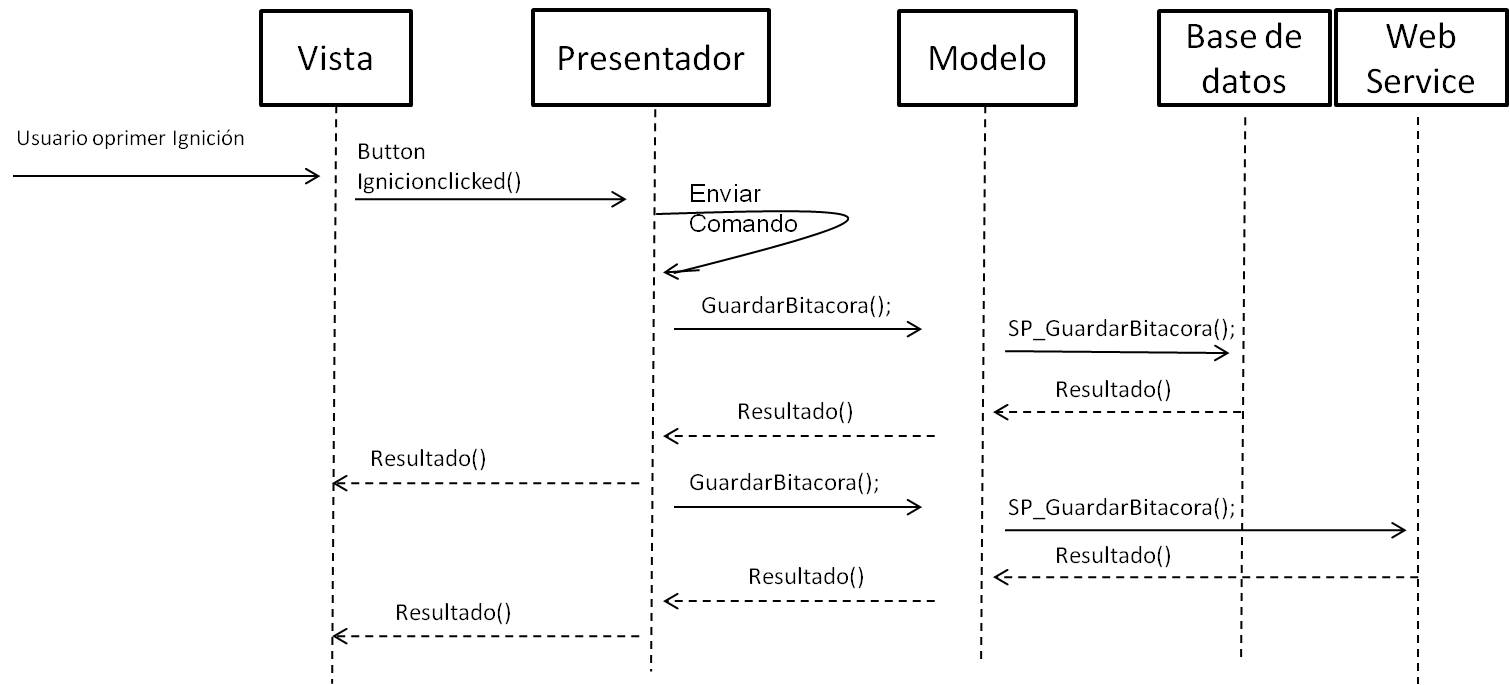
\includegraphics[width=0.95\textwidth]{metodologia/DSIgnicion.jpg}
\caption{Diagrama de secuencia del flujo de la funcionalidad ignición para el encendido automatico.}
\label{ds11}
\end{figure}
%
 \begin{enumerate}
\item El usuario selecciona la opción encendido automatico ignición.
\item La capa de presentador toma la información de la opción seleccionada y la envia via Bluetooth a la tarjeta electrónica y espera una respuesta de la tarjeta electrónica por el mismo medio de comunicación.
\item Después de adquirir la respuesta envia a la pantalla un mensaje.
\item La capa presentador envia una petición de guardado hacia la base de datos para el registro de las actividades en la aplicación formando un historial, al igual que envia la información de la bitacora hacia el servicio web para crear un registro de la aplicación en linea.
\end{enumerate}

La Figura \ref{ds12} se muestra el evento de la secuencia de arrancar la marcha para el encendido automatico.\\
\begin{figure}[H]
%\vspace{0.2cm}
\centering
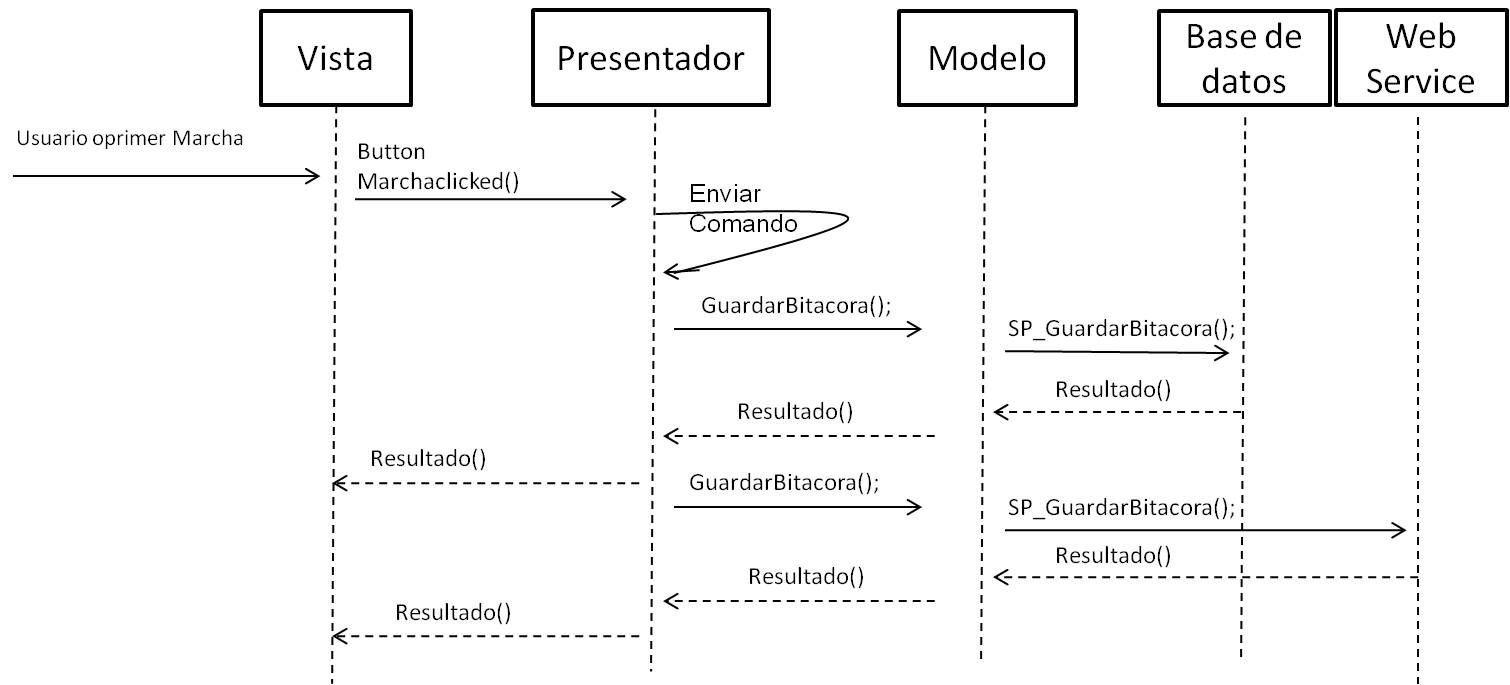
\includegraphics[width=0.95\textwidth]{metodologia/DSMarcha.jpg}
\caption{Diagrama de secuencia del flujo de la funcionalidad marcha para el encendido autoamtico.}
\label{ds12}
\end{figure}
%
 \begin{enumerate}
\item El usuario selecciona la opción encendido automatico marcha.
\item La capa de presentador toma la información de la opción seleccionada y la envia via Bluetooth a la tarjeta electrónica y espera una respuesta de la tarjeta electrónica por el mismo medio de comunicación.
\item Después de adquirir la respuesta envia a la pantalla un mensaje.
\item La capa presentador envia una petición de guardado hacia la base de datos para el registro de las actividades en la aplicación formando un historial, al igual que envia la información de la bitacora hacia el servicio web para crear un registro de la aplicación en linea.
\end{enumerate}

Se realizó una configuración para el envio de información desde el dispositivo móvil con un servicio Web, este servicio nos permitirá conocer las actividades que realiza el usuario, a su vez nos ayudarán a automatizar nuevas funcionalidades y a visualizar las necesidades del usuario según su historial de funcionalidad. El funcionamiento de la comunicación entre la aplicación y el servicio Web de muestra en la Figura \ref{webservice}. Estás bitácoras se visualizan desde el servidor mediante una aplicación Web, tal cual se muestra en la Figura \ref{bitacoraweb}


\begin{figure}[H]
%\vspace{0.2cm}
\centering
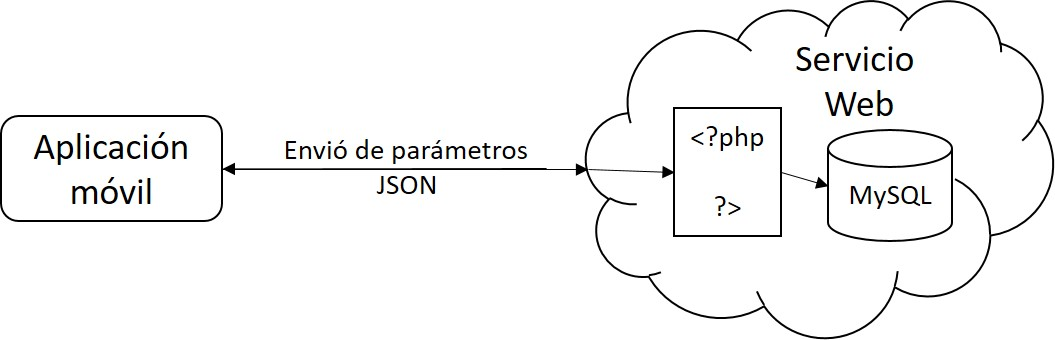
\includegraphics[width=0.95\textwidth]{metodologia/webservice.jpg}
\caption{Comunicación entre la aplicación móvil y el servicio Web.}
\label{webservice}
\end{figure}
%

\begin{figure}[H]
%\vspace{0.2cm}
\centering
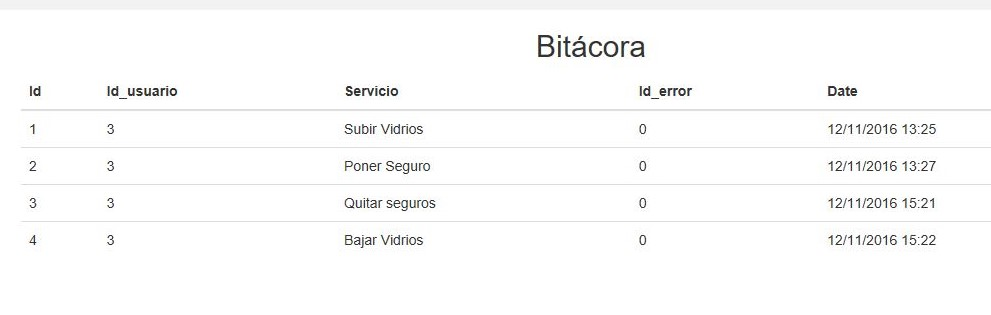
\includegraphics[width=0.95\textwidth]{aplicacion/bitacoraweb.jpg}
\caption{Aplicación para visualizar el historial de los usuarios.}
\label{bitacoraweb}
\end{figure}


El proceso de instalación del archivo .apk se enumera en la siguiente lista: \\
\begin{enumerate}
\item descargar el archivo.
\item acceder a ajustes despúes a Pantalla bloqueo/seguridad.
\item permitir fuentes desconocidas.
\item abrir el archivo descargado.
\item seleccionar la opción instalar.
\item esperar a que se instale.
\item presionar el botón Hecho o abrir.

\end{enumerate}



El funcionamiento de la aplicación móvil es el siguiente. Lo primero que aparece es solicitar el usuario y la contraseña tal como se muestra en la Figura \ref{login1} incisos a, b y c, en donde se pone un bloque de seguridad para evitar accesos no deseados.

\begin{figure}[H]
\centering
\subfigure[]{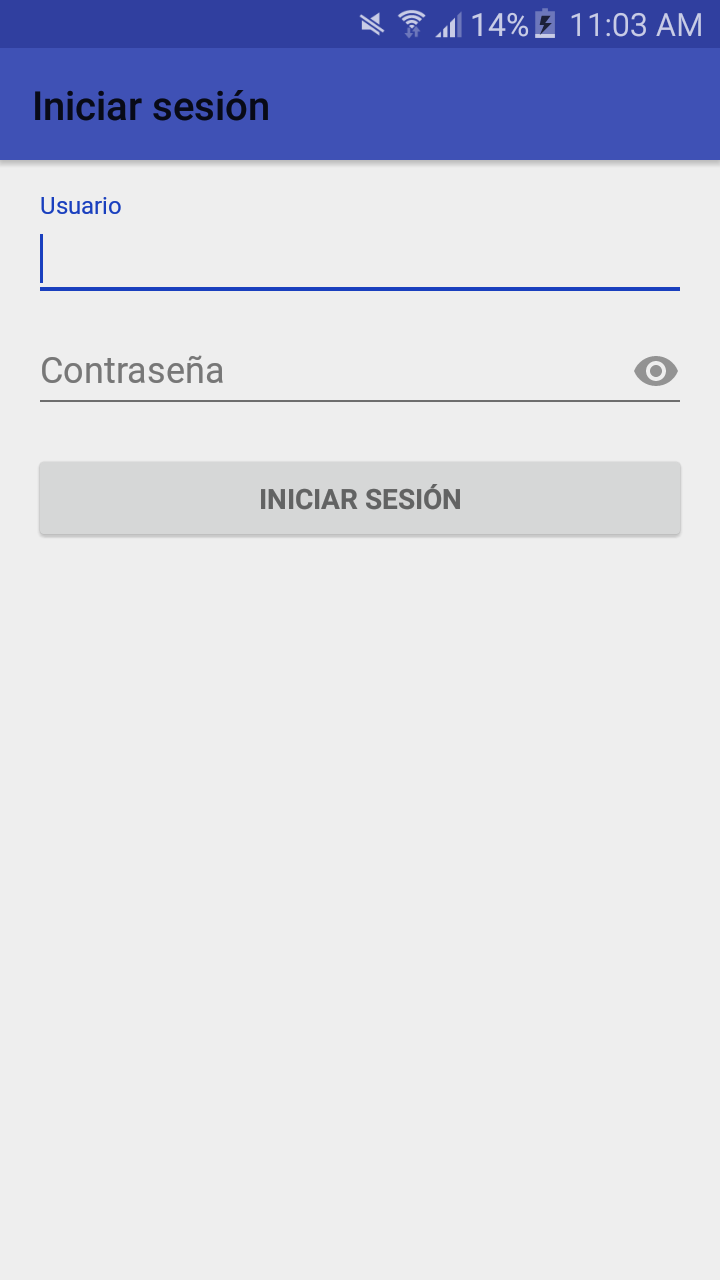
\includegraphics[width=50mm]{aplicacion/login1.jpg}}\hspace{5mm}
\subfigure[]{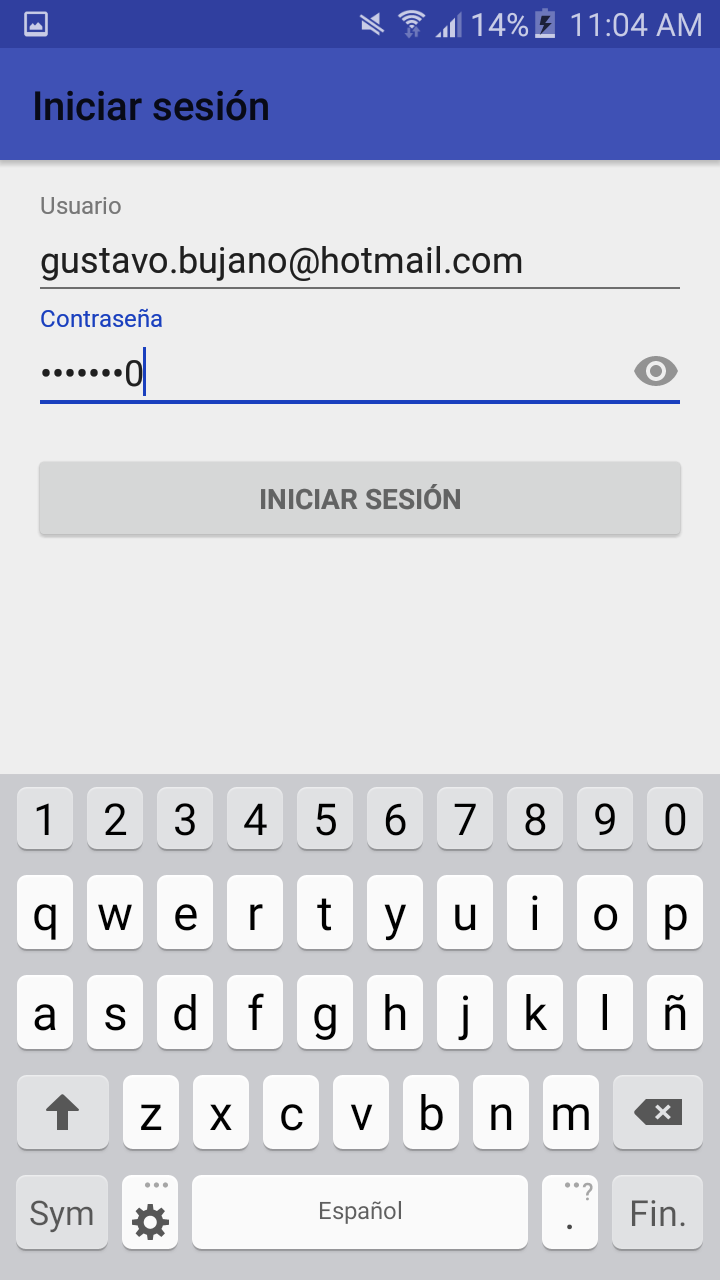
\includegraphics[width=50mm]{aplicacion/login2.jpg}}\hspace{5mm}
\subfigure[]{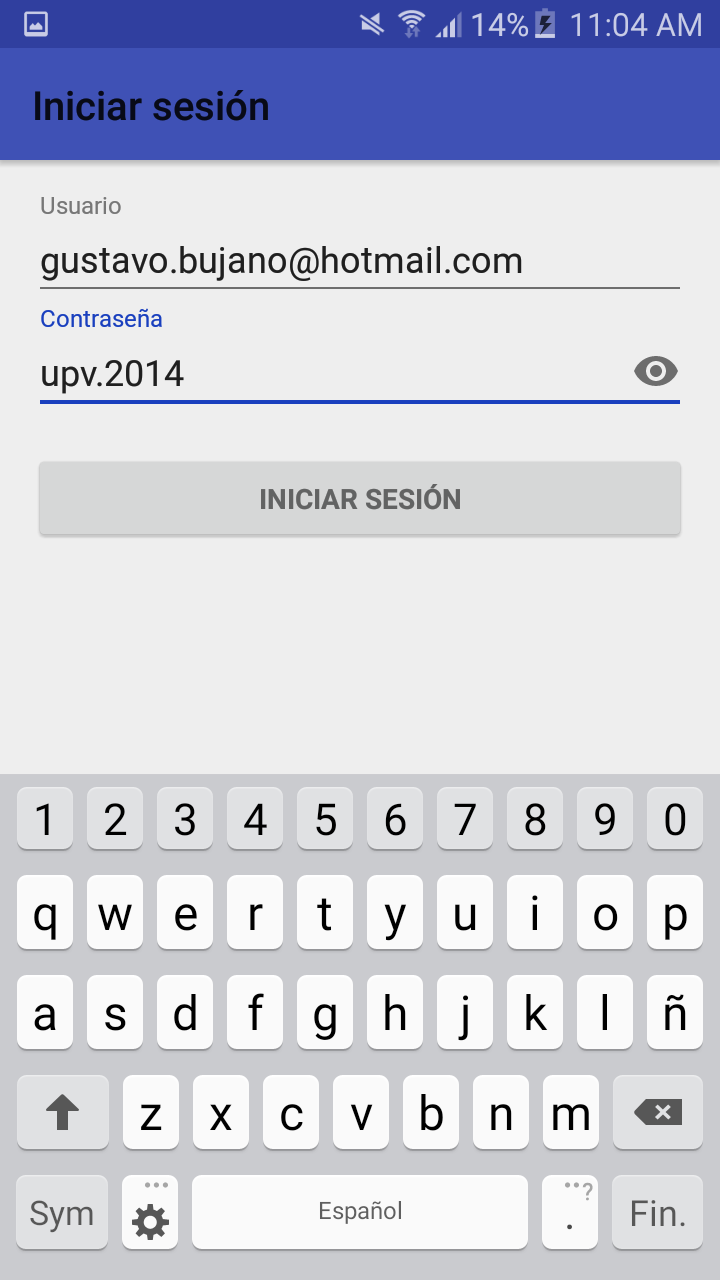
\includegraphics[width=50mm]{aplicacion/login3.jpg}}\hspace{5mm}
\caption{Login de la aplicación.}
\label{login1}
\end{figure}

Una vez ingresado el usuario y la contraseña de manera correcta se mostrará una pantalla principal, en ella se muestra si se encuentra activado el \textit{Bluetooth} ver Figura \ref{principal} inciso a, en caso de no estar activado, la aplicación de manera automática activa el \textit{Bluetooth}, ver Figura \ref{principal} inciso b, y queda a la espera de que el usuario, para desactivar el \textit{Bluetooth} el usuario necesita oprimir el boton con el icono simplemente.\\

\begin{figure}[H]
\centering
\subfigure[]{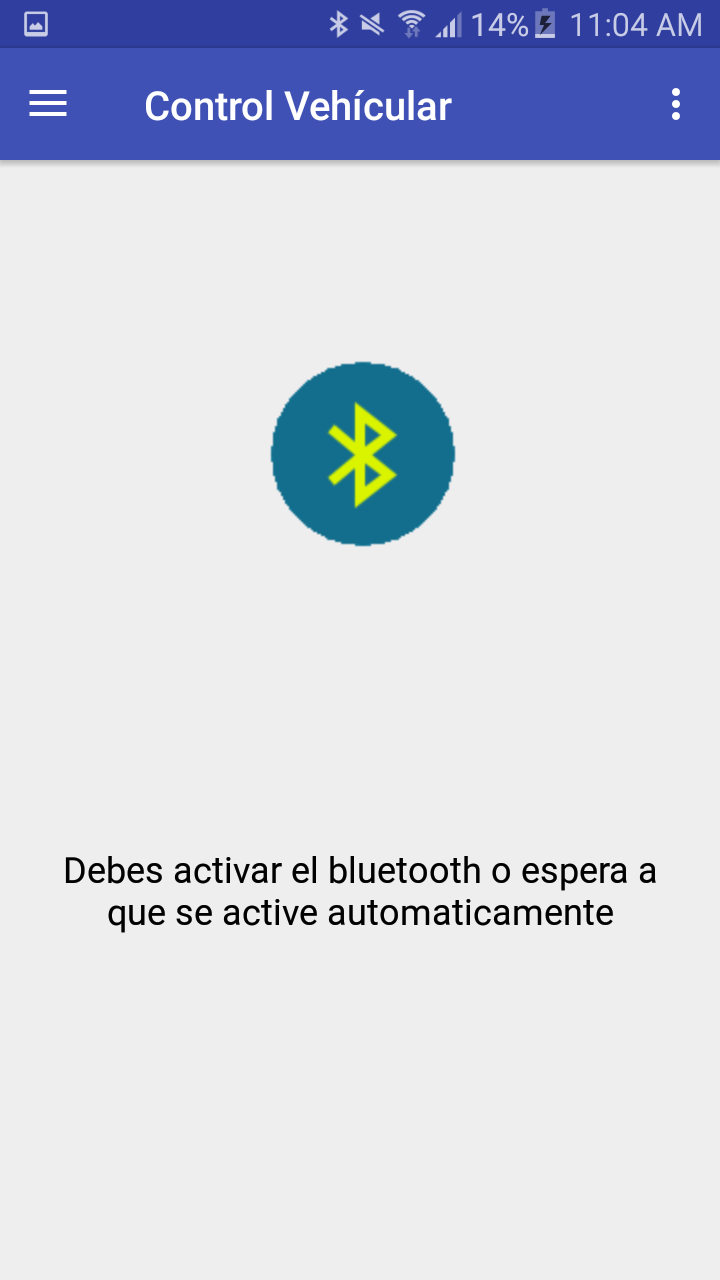
\includegraphics[width=50mm]{aplicacion/principal1.jpg}}\hspace{5mm}
\subfigure[]{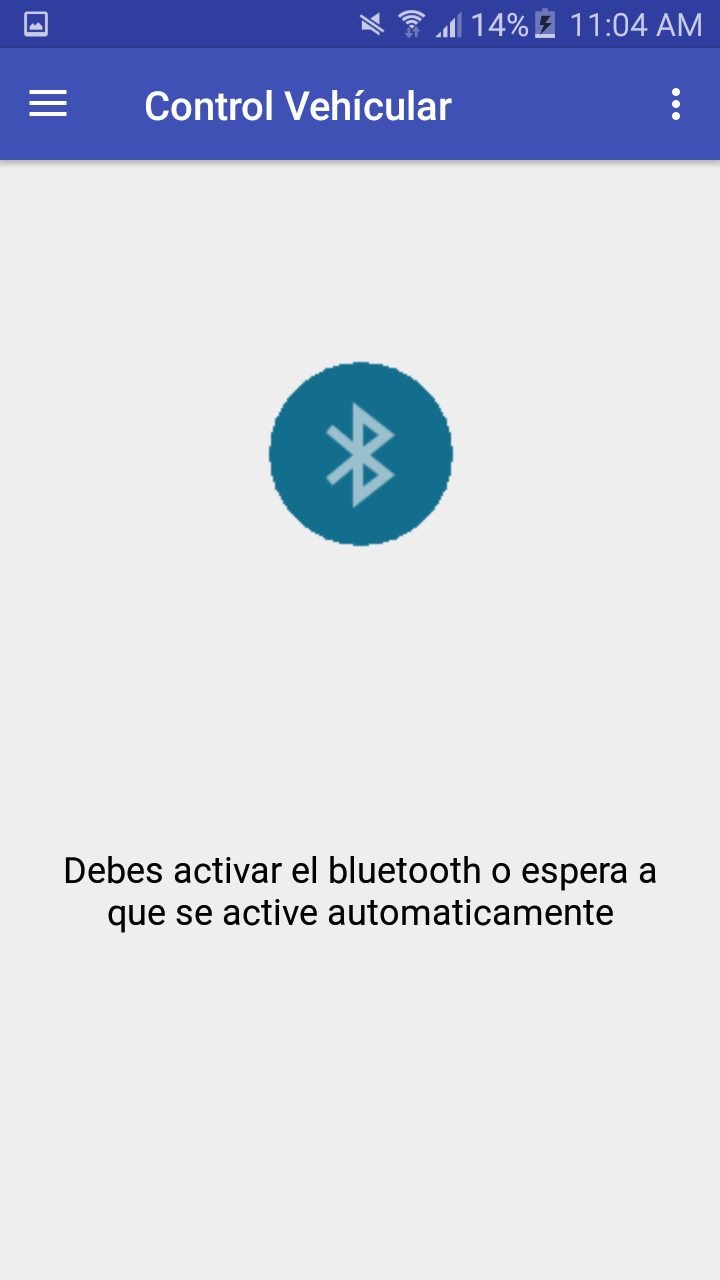
\includegraphics[width=50mm]{aplicacion/principal2.jpg}}\hspace{5mm}
\caption{Pantalla principal de la aplicación.}
\label{principal}
\end{figure}

Dentro de la pantalla principal el sistema cuenta con un menu oculto que se encuentra del lado superior izquierdo, tal cual se muestra en la Figura\ref{menu}. Por otro lado del lado derecho la aplicación cuenta con funcionalidades de preferencia, como: cambiar contraseña, cerrar sesion y ayuda ver Figura \ref{preferencias}.

%
\begin{figure}[H]
%\vspace{0.2cm}
\centering
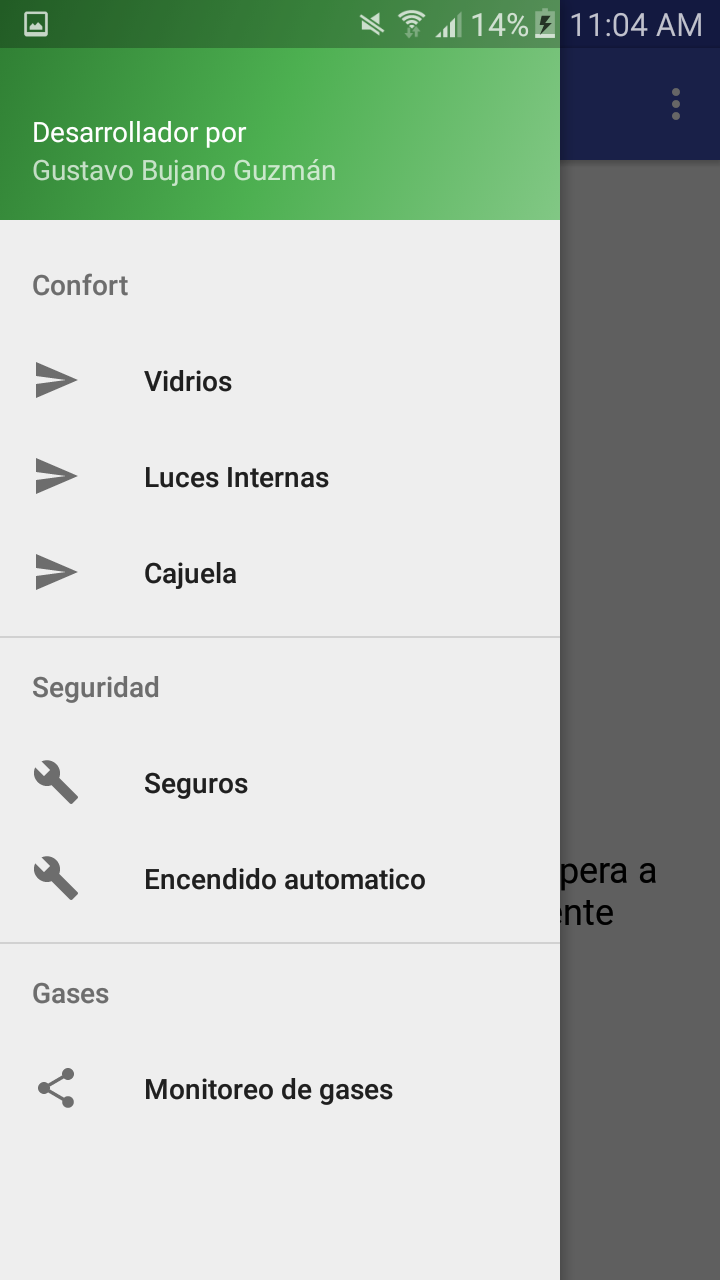
\includegraphics[width=0.4\textwidth]{aplicacion/menu.jpg}
\caption{Menu de opciones de la aplicación.}
\label{menu}
\end{figure}

%
\begin{figure}[H]
%\vspace{0.2cm}
\centering
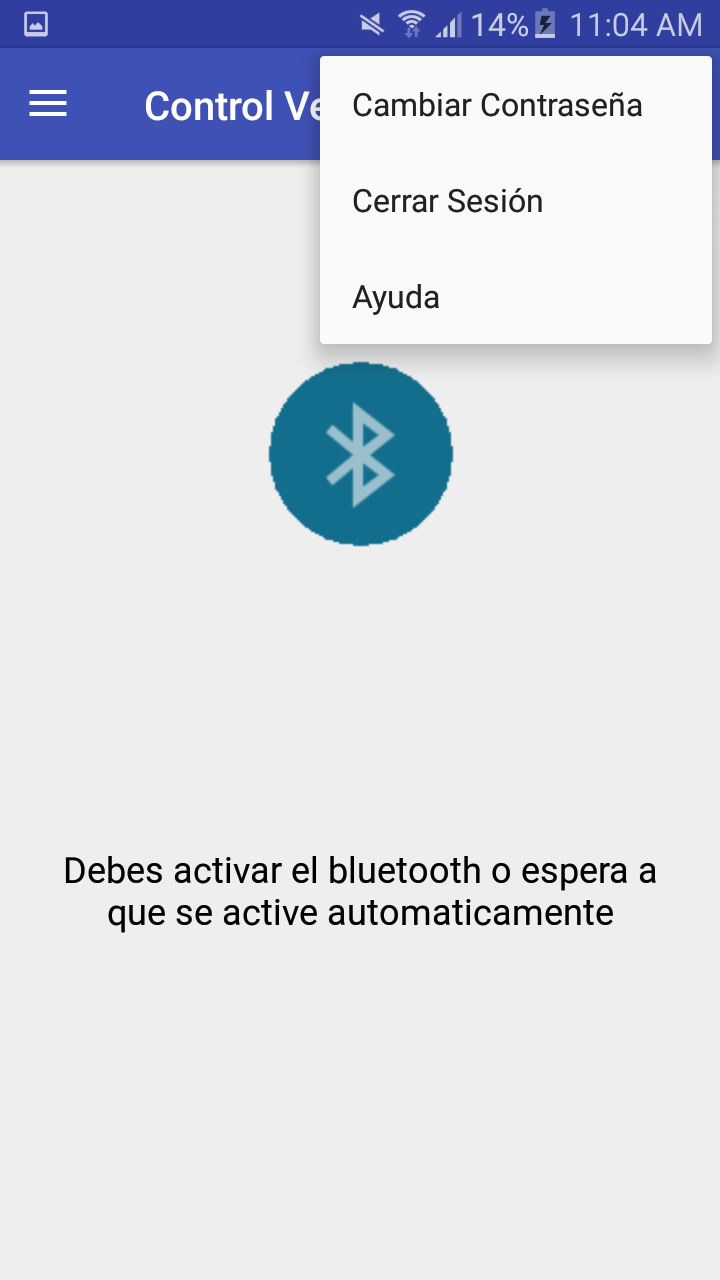
\includegraphics[width=0.4\textwidth]{aplicacion/preferencias.jpg}
\caption{Menu de preferencias de la aplicación.}
\label{preferencias}
\end{figure}

Dentro del menu, se encuentran todas las funcionalidades hacia el vehículo, englobados  por 4 secciones, a)confort, b)seguridad, c) gases y d) Otros:
 \begin{enumerate}
\item Funcionalidad de vidrios electrícos, Ver Figura \ref{vidrios}. En esta pantalla el usuario puede enviar la señal para bajar el vidrios como se muestra en el incisoa, o subir un vidrio tal cual se muestran en el inciso b.


\begin{figure}[H]
\centering
\subfigure[]{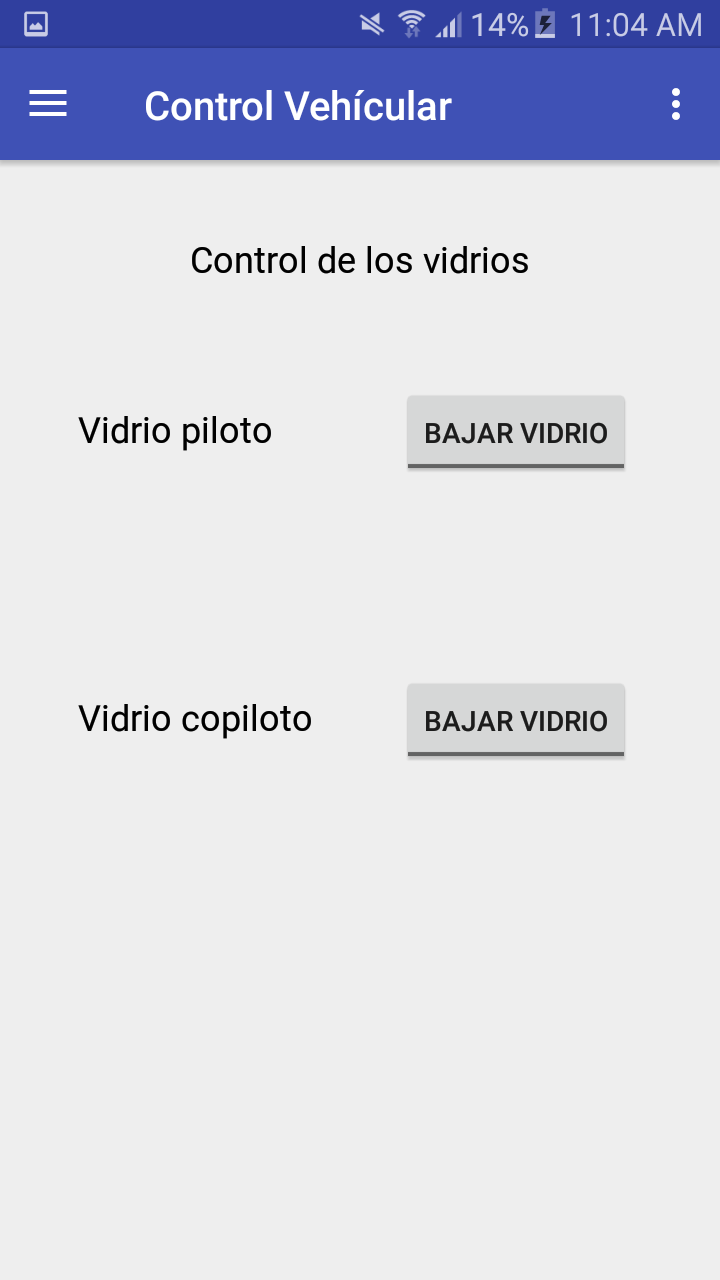
\includegraphics[width=50mm]{aplicacion/vidrios.jpg}}\hspace{5mm}
\subfigure[]{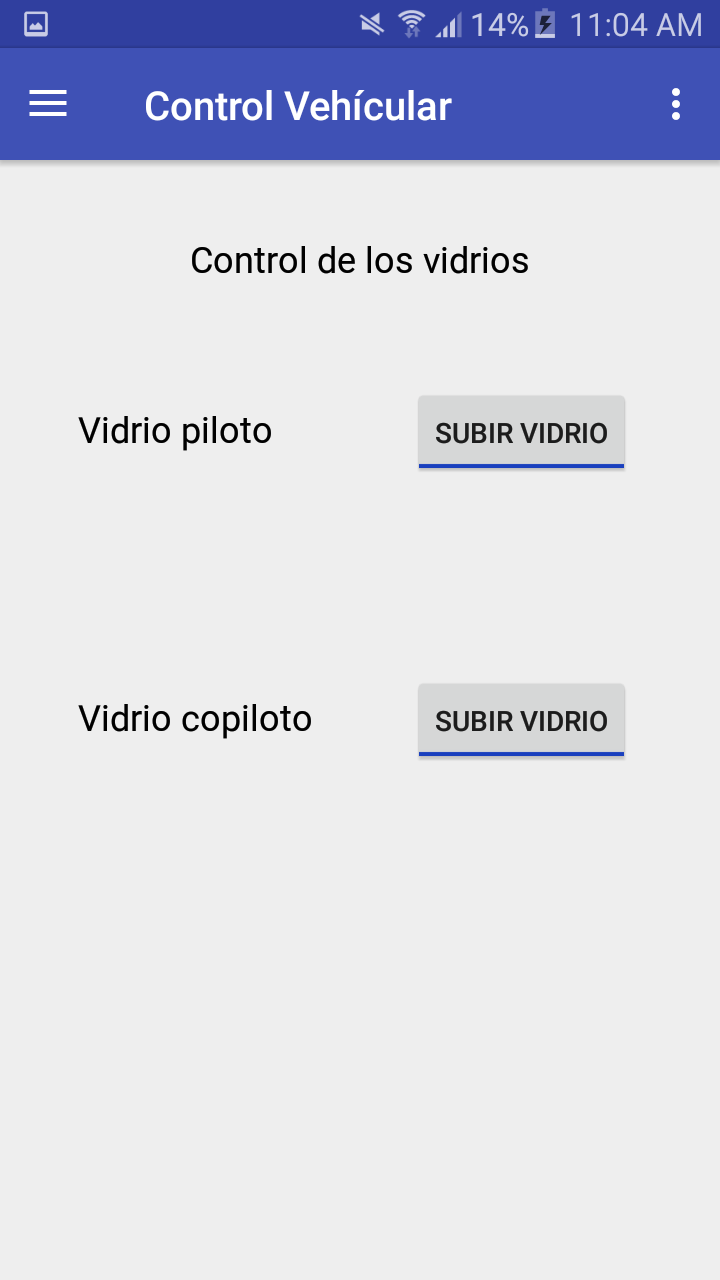
\includegraphics[width=50mm]{aplicacion/vidrios2.jpg}}\hspace{5mm}
\caption{Pantalla del la funcionalidad para los vidrios electrícos.}
\label{vidrios}
\end{figure}

\item Funcionalidad de luces, ver Figura \ref{luces}. En esta pantalla el usuario puede enviar la señal para activar o desactivar las luces, tanto internas ver inciso a, y externas ver inciso b.

\begin{figure}[H]
\centering
\subfigure[]{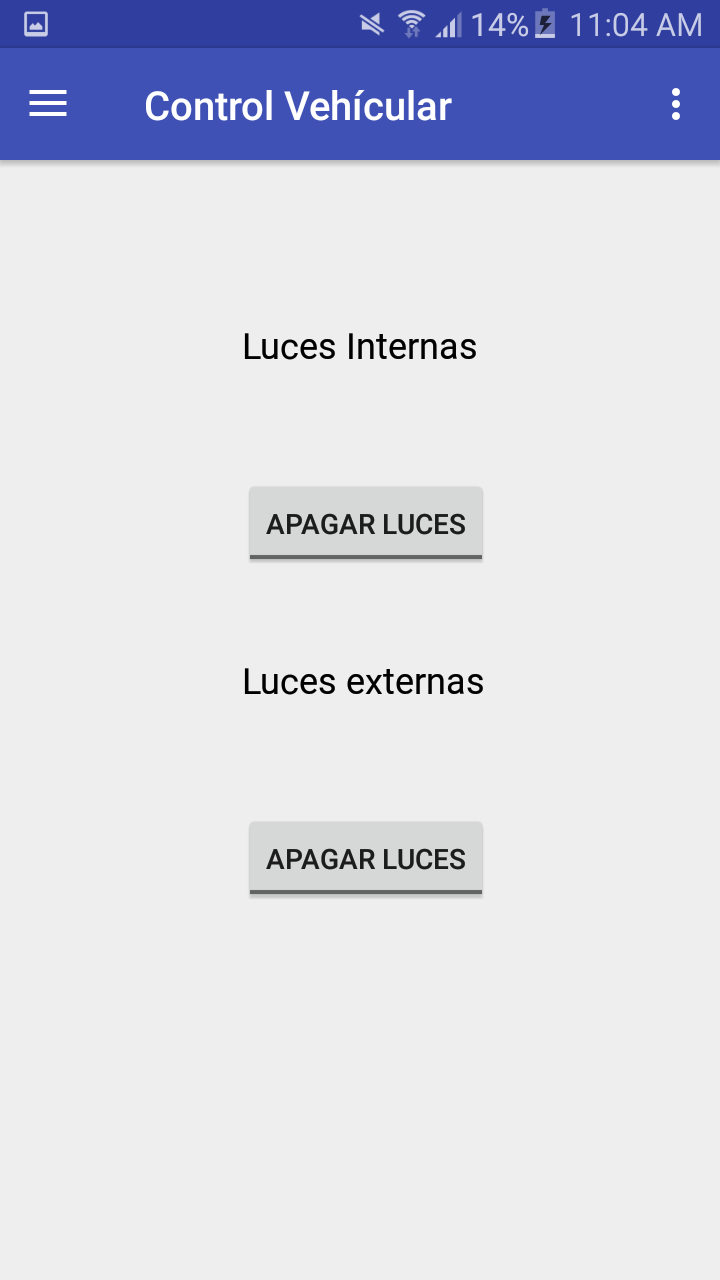
\includegraphics[width=50mm]{aplicacion/luces.jpg}}\hspace{5mm}
\subfigure[]{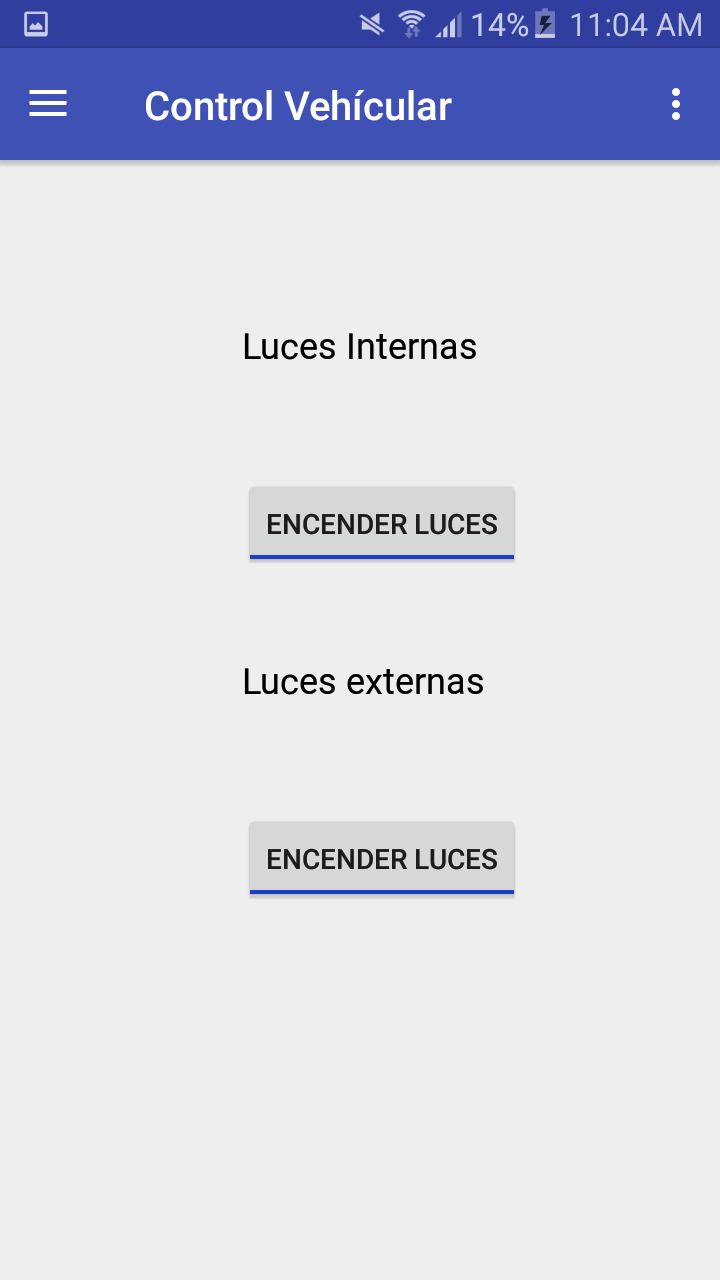
\includegraphics[width=50mm]{aplicacion/luces2.jpg}}\hspace{5mm}
\caption{Pantalla del la funcionalidad para las luces.}
\label{luces}
\end{figure}

\item Funcionalidad de cajuela, ver Figura \ref{cajuela}. En esta pantalla el usuario puede enviar la señal para activar el desbloqueo de la cajuela.

\begin{figure}[H]
\centering
\subfigure[]{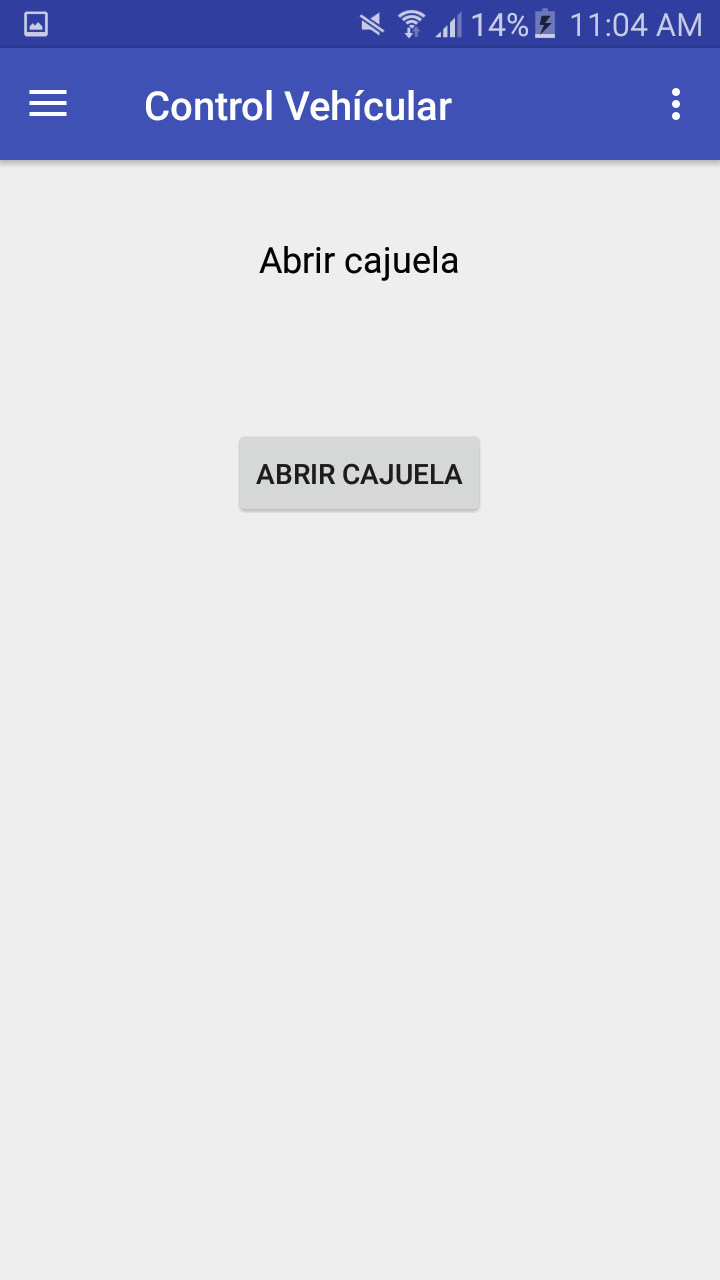
\includegraphics[width=50mm]{aplicacion/cajuela.jpg}}\hspace{5mm}
\caption{Pantalla del la funcionalidad para la cajuela.}
\label{cajuela}
\end{figure}

\item Funcionalidad de seguros. Ver Figura \ref{seguros}. En esta pantalla el usuario puede enviar la señal para activar o desactivar los seguros de las puertas.

\begin{figure}[H]
\centering
\subfigure[]{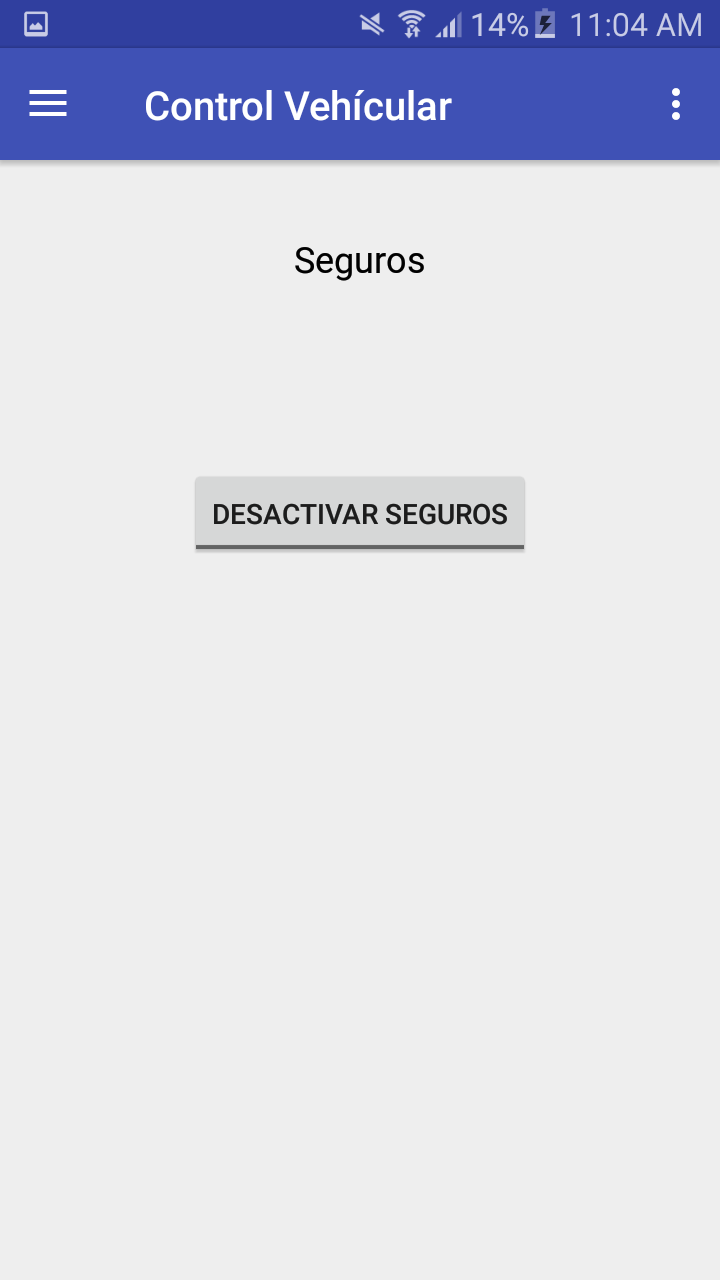
\includegraphics[width=50mm]{aplicacion/seguros.jpg}}\hspace{5mm}
\caption{Pantalla del la funcionalidad para los seguros de las puertas.}
\label{seguros}
\end{figure}

\item Funcionalidad de encendido automatico, ver Figura \ref{encendido}. Esta funcionalidad permite activar la ignición y posteriormente se podrá activar la marcha 2 segundos para que el vehículo pueda encender.
\begin{figure}[H]
\centering
\subfigure[]{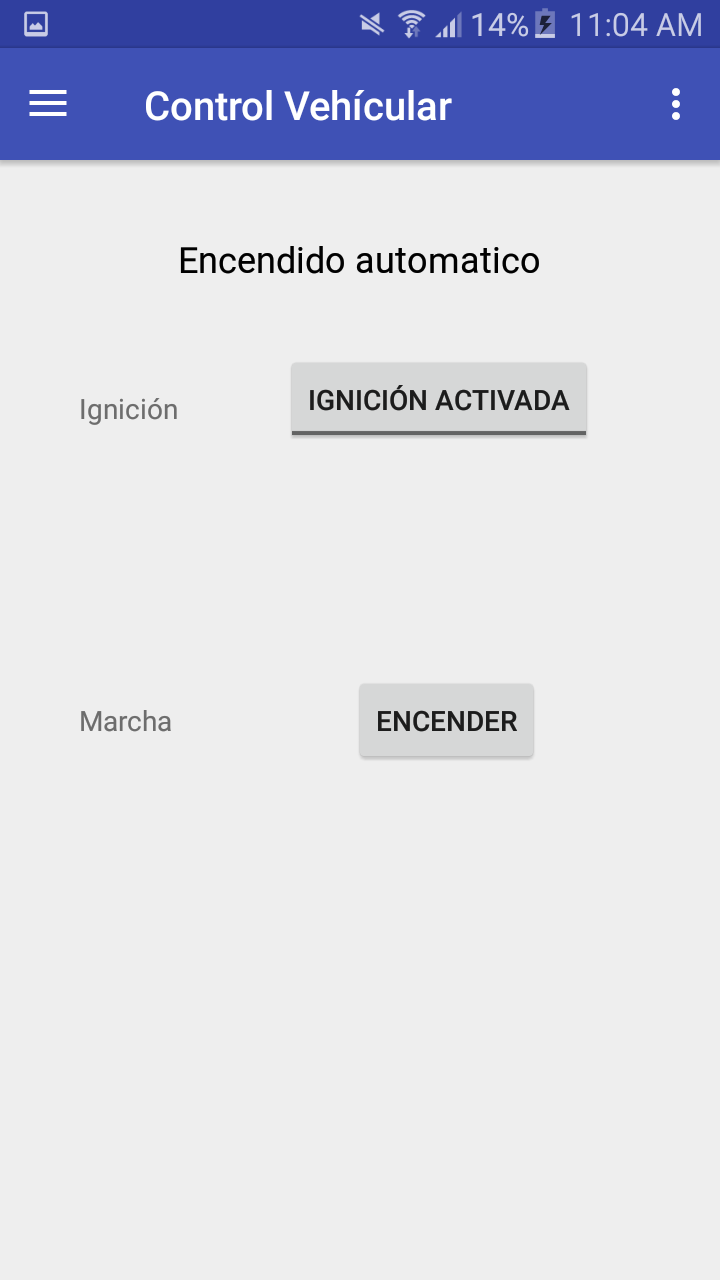
\includegraphics[width=50mm]{aplicacion/encendido.jpg}}\hspace{5mm}
\subfigure[]{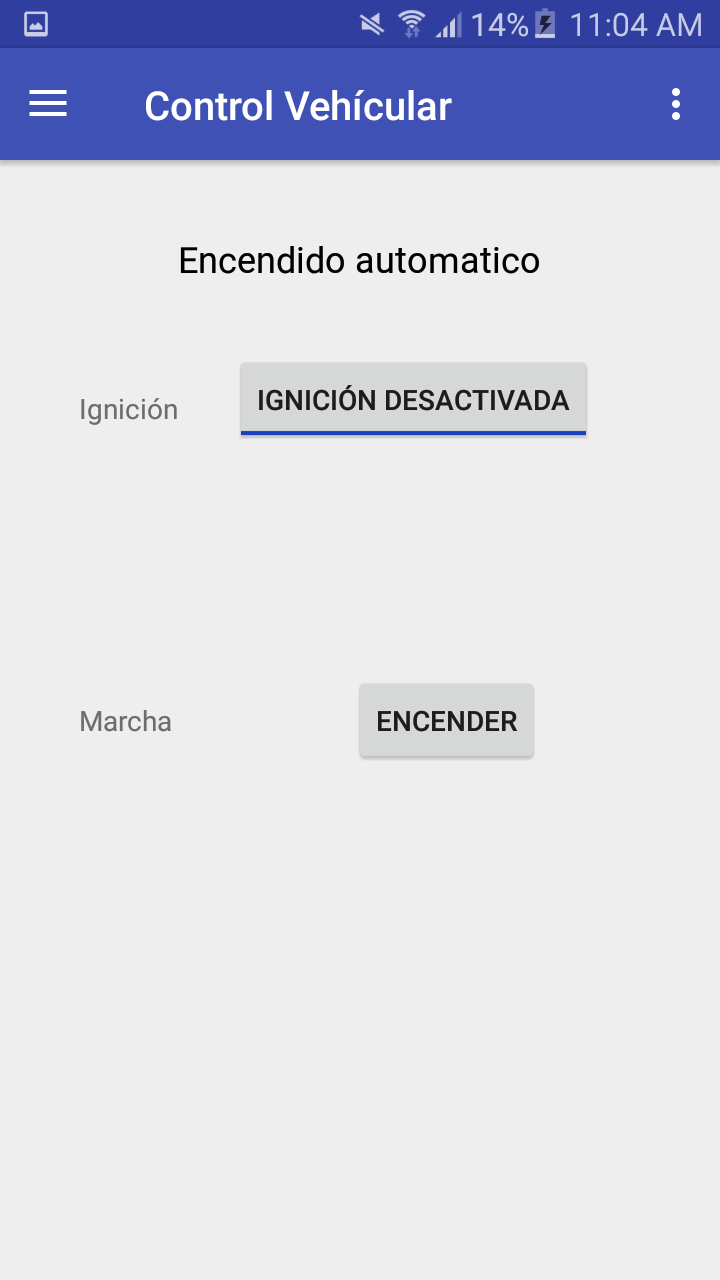
\includegraphics[width=50mm]{aplicacion/encendido2.jpg}}\hspace{5mm}
\caption{Pantalla del la funcionalidad para el encendido automatico.}
\label{encendido}
\end{figure}

\item Funcionalidad de monitoreo de gases, ver Figura \ref{monitoreo}. Esta funcionalidad permite visualizar los niveles de óxido de nitrógeno del vehículo.

\begin{figure}[H]
\centering
\subfigure[]{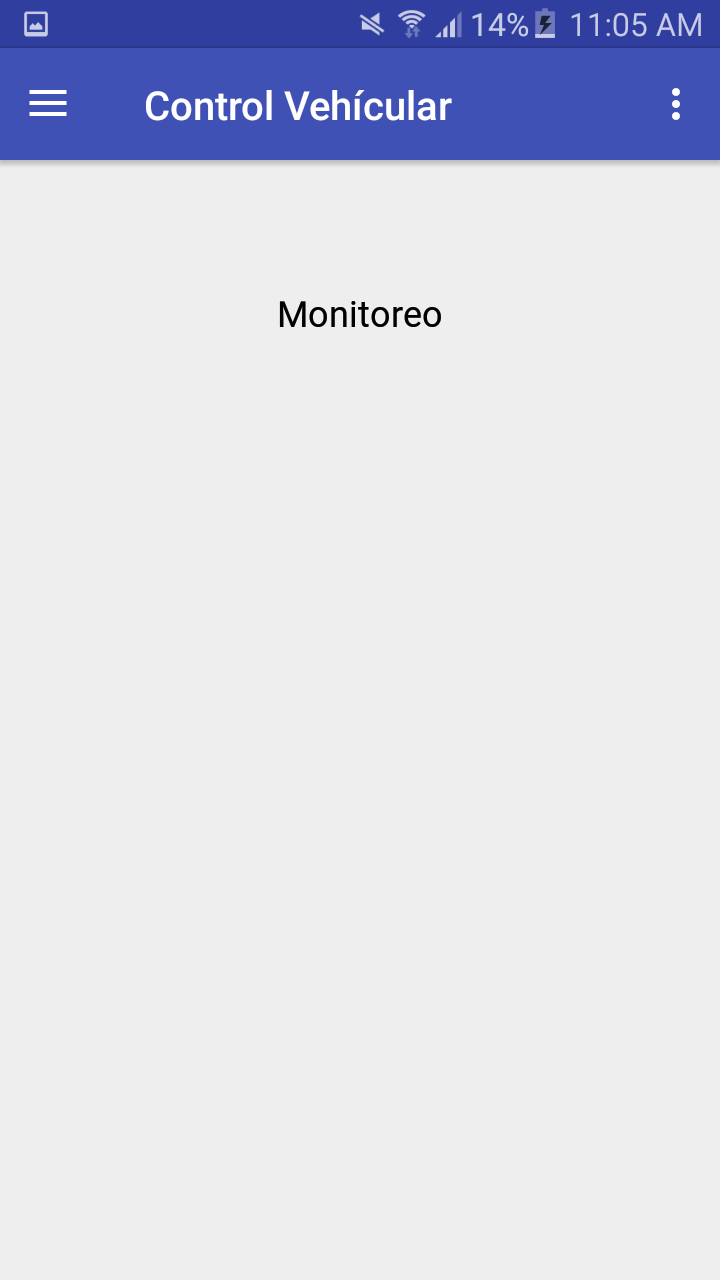
\includegraphics[width=50mm]{aplicacion/monitore.jpg}}\hspace{5mm}
\caption{Pantalla del la funcionalidad para el monitoreo de óxido de Nitrógeno.}
\label{monitoreo}
\end{figure}

\item Funcionalidad de comandos automáticos, ver Figura  \ref{comandos}. Esta funcionalidad permite ejecutar dos o más comandos en secuencia. En este caso se encuentra un comando automático, poner seguro a las puertas y subir los vidrios.

\begin{figure}[H]
\centering
\subfigure[]{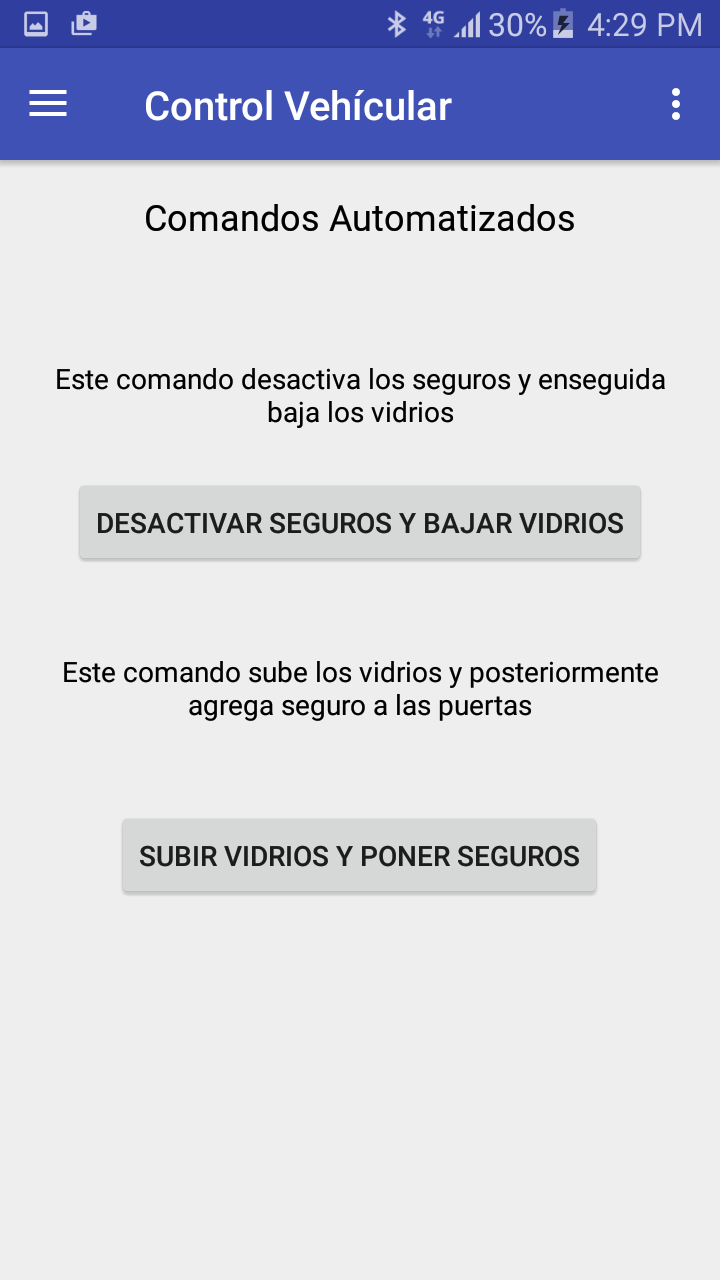
\includegraphics[width=50mm]{aplicacion/comandos.jpg}}\hspace{5mm}
\caption{Pantalla del la funcionalidad para comandos automátizados.}
\label{comandos}
\end{figure}

\item Funcionalidad de Bitácora, ver Figura \ref{bitacora}. Esta funcionalidad permite mostrar todos los comandos que se han ejecutado en la aplicación.
\begin{figure}[H]
\centering
\subfigure[]{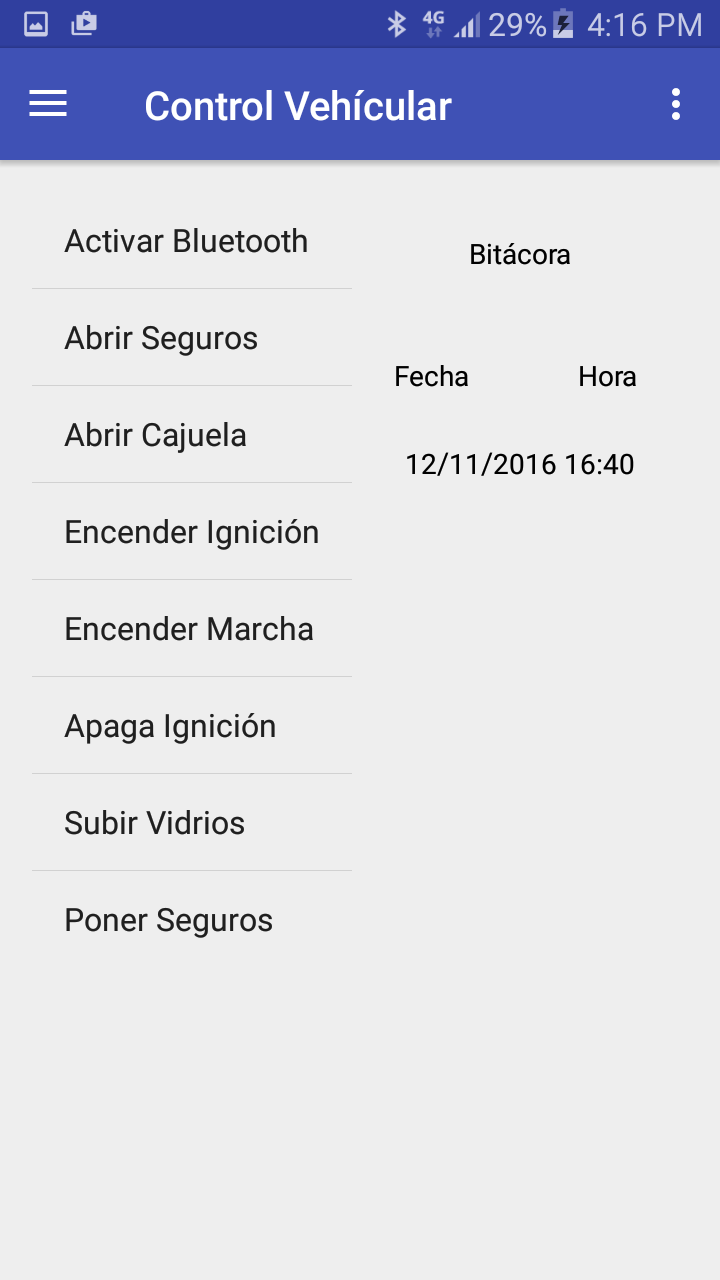
\includegraphics[width=50mm]{aplicacion/bitacora.jpg}}\hspace{5mm}
\caption{Pantalla del la funcionalidad bitácora.}
\label{bitacora}
\end{figure}

\end{enumerate}











\subsection{CONECTIVIDAD}

Bluetooth es la tecnología que se ha seleccionado para realizar la conectividad debido a su tendencia en la comunicación inalámbrica y su compatibilidad. Actualmente los dispositivos móviles ya cuentan con esta tecnología. Por otra parte, se le ha conectado a la tarjeta electrónica el \textit{shield} Bluetooth HC-05 tal cual se muestra en las Figuras \ref{conexion} y \ref{conexion2}\\


%
\begin{figure}[H]
%\vspace{0.2cm}
\centering
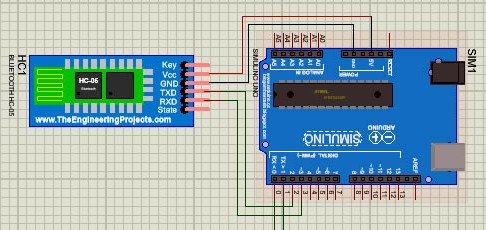
\includegraphics[width=0.8\textwidth]{metodologia/conexion_bluetooth2.jpg}
\caption{Simulación de la conexión de la tarjeta electrónica y el \textit{shild} Bluetooth}
\label{conexion2}
\end{figure}

%
\begin{figure}[H]
%\vspace{0.2cm}
\centering
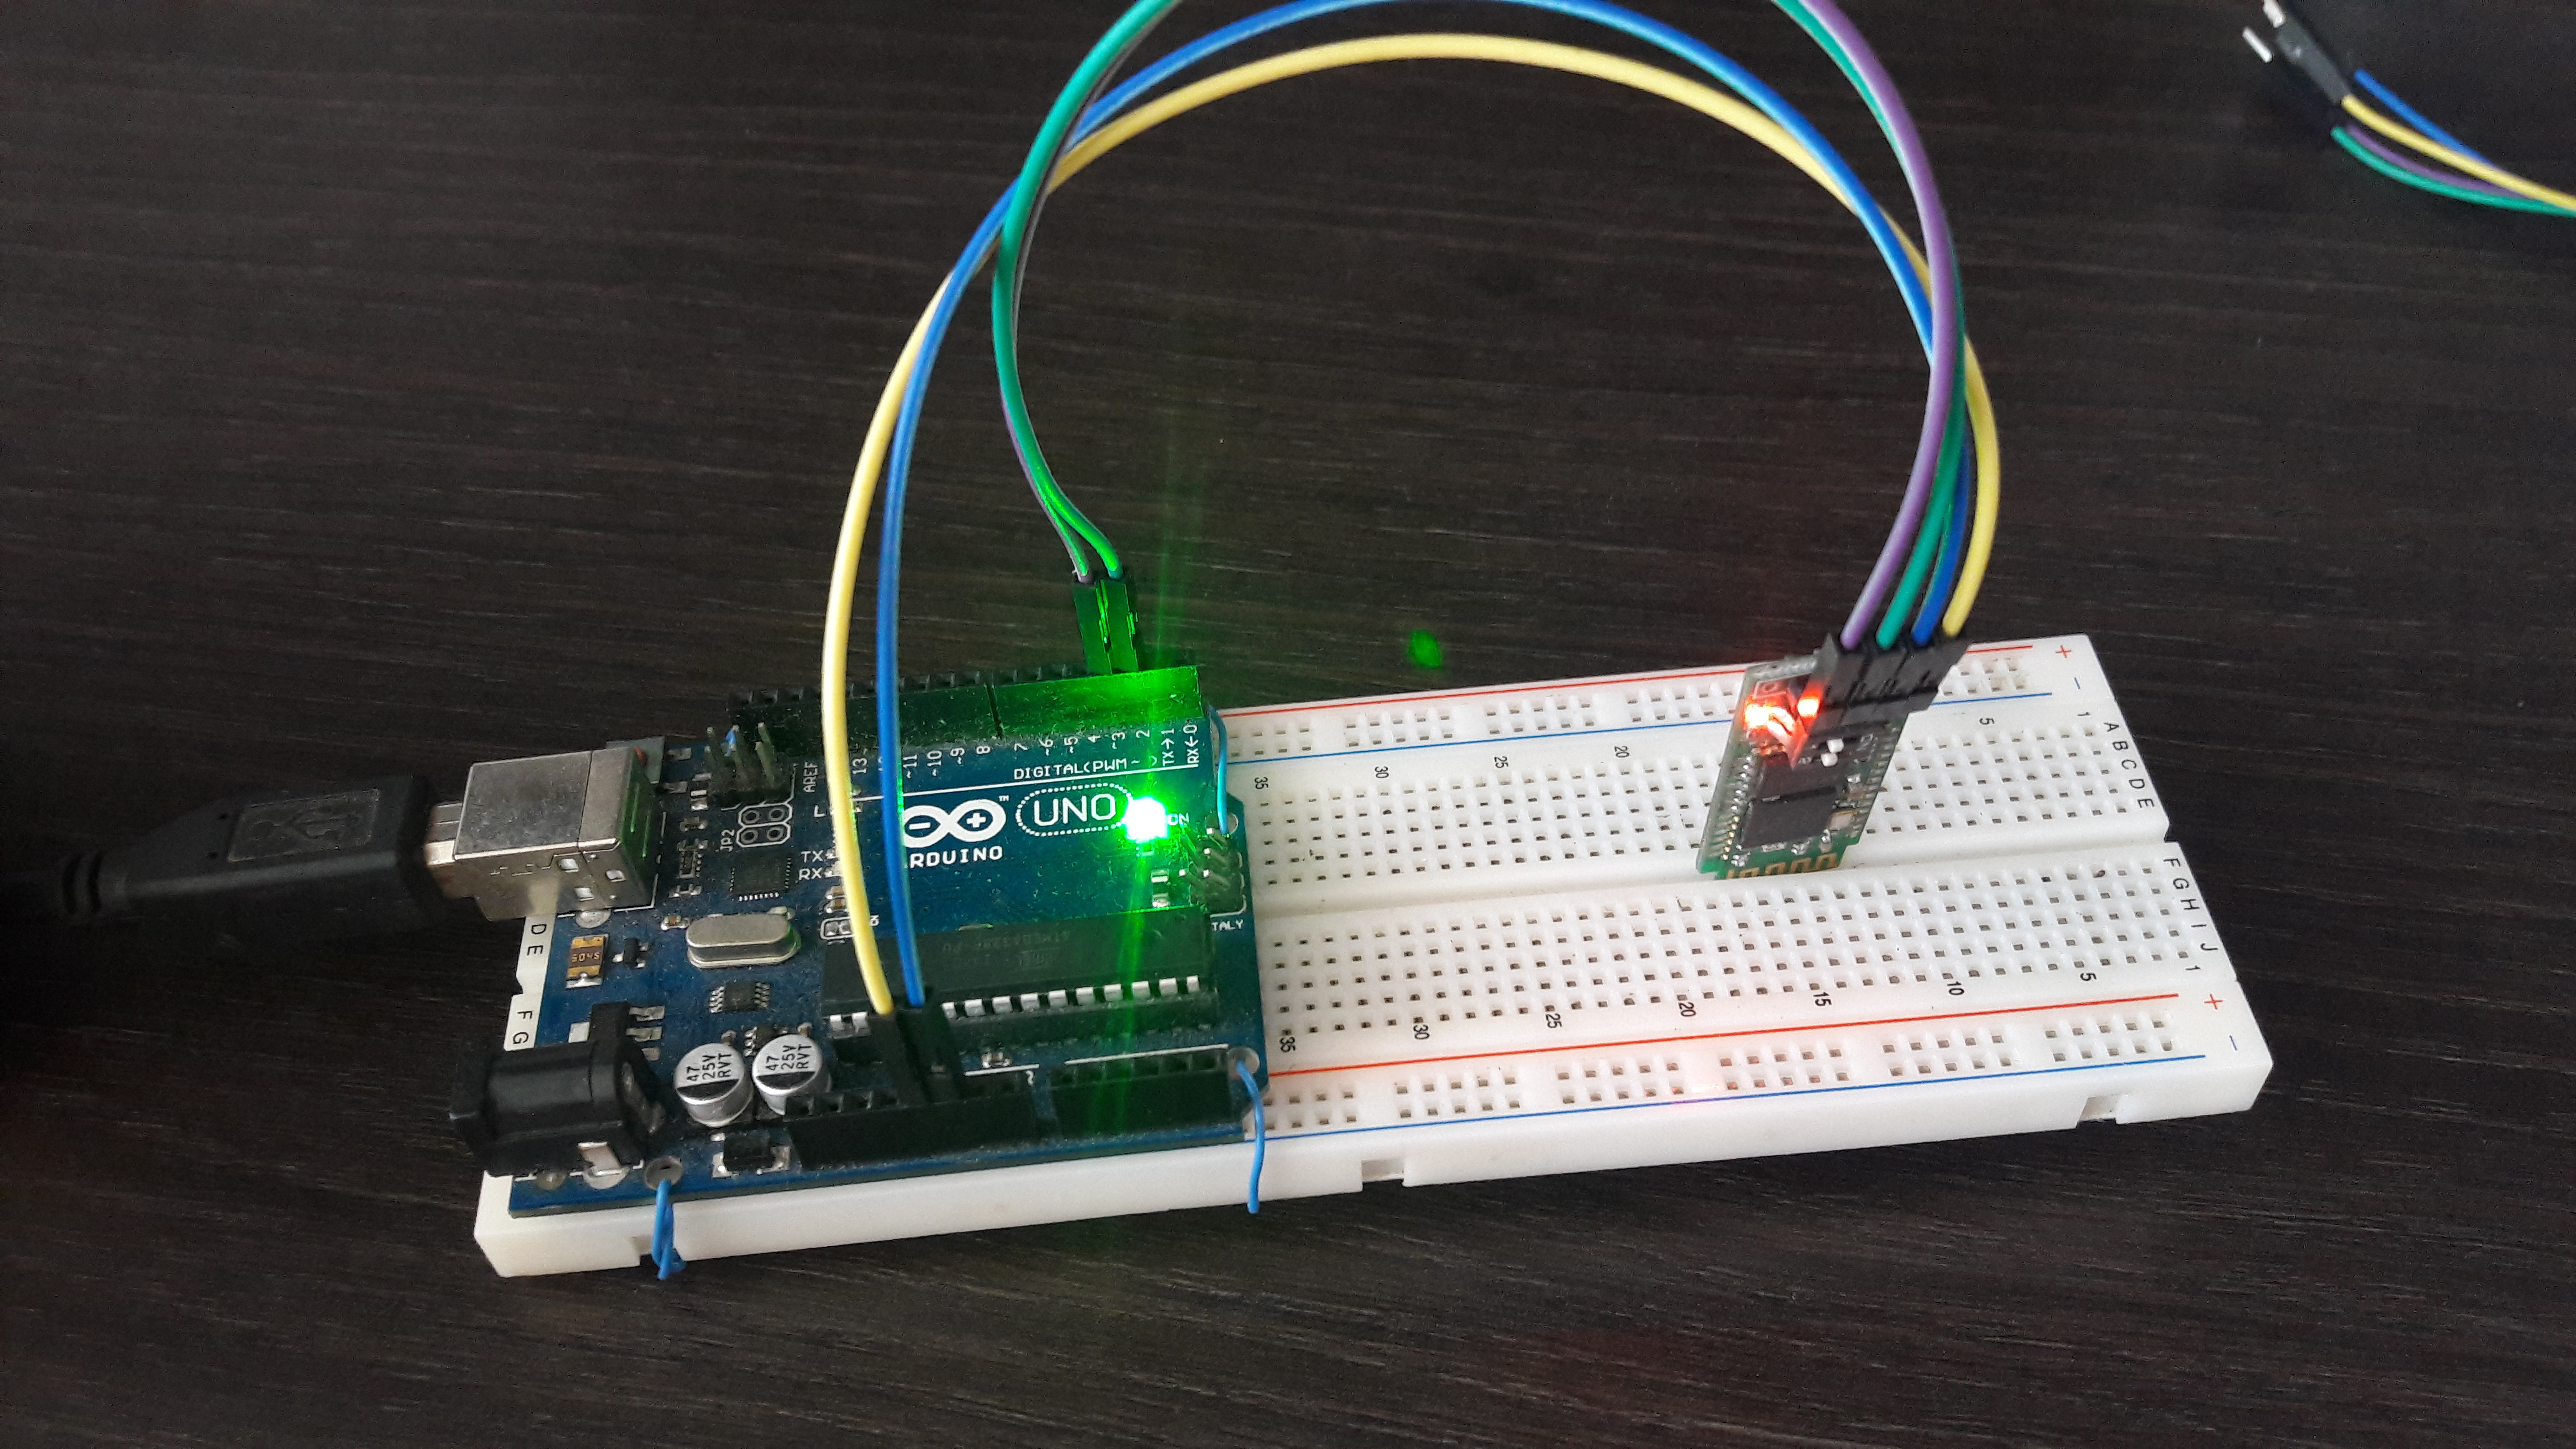
\includegraphics[width=0.8\textwidth]{metodologia/conexion_bluetooth.jpg}
\caption{Conexión de la tarjeta electrónica y el \textit{shild} Bluetooth}
\label{conexion}
\end{figure}


El proceso de conexión entre el disositivo móvil y la tarjeta electrónica por primera vez se muestra a continuación:

\begin{enumerate}
\item Activar la tarjeta electrónica para que se active el shield bluetooth.
\item Activar el bluetooth del dispositivo móvil.
\item Acceder a la configuración del bluetooth del disposito.
\item Seleccionar en dispositivo disponible el preferido (ver Figura \ref{vinc} inciso a).
\item Introducir el PIN para vincular el dispositivo (ver Figura \ref{vinc} inciso b).
\item El dispositivo se mostrará vinculado (ver Figura \ref{vinc} inciso c).
\end{enumerate}

\begin{figure}[H]
\centering
\subfigure[]{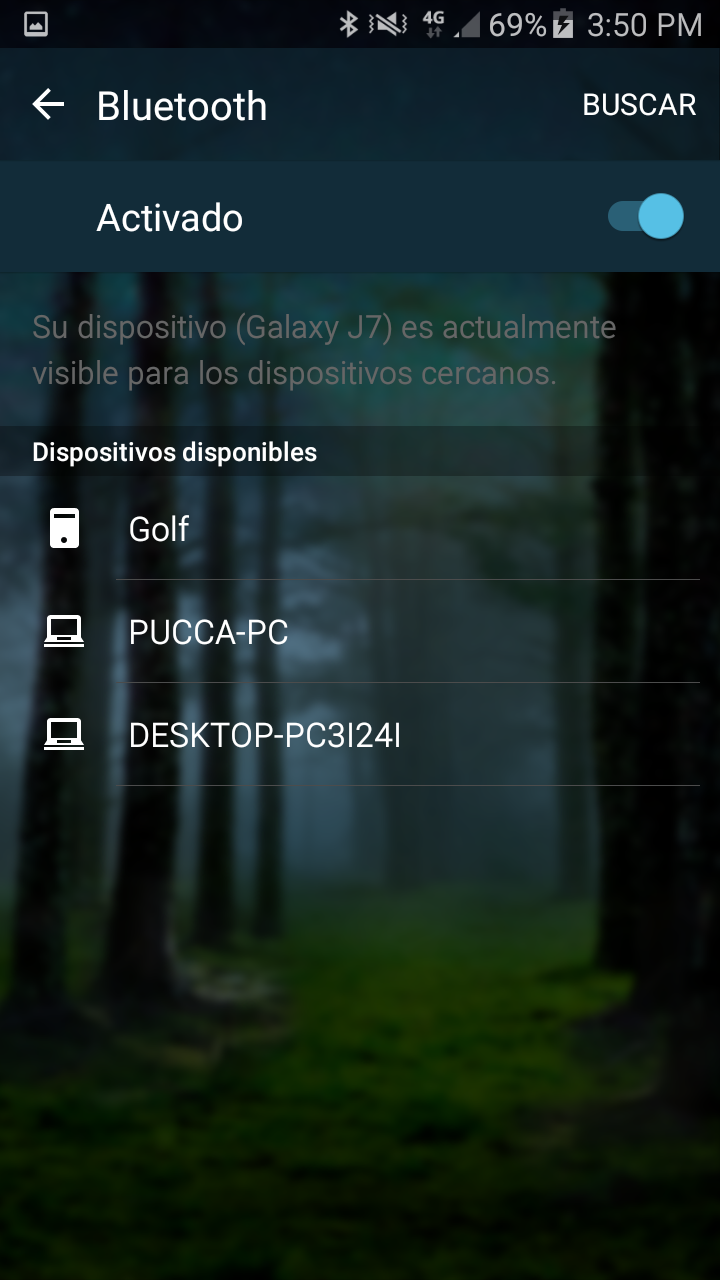
\includegraphics[width=50mm]{metodologia/vinc.png}}\hspace{5mm}
\subfigure[]{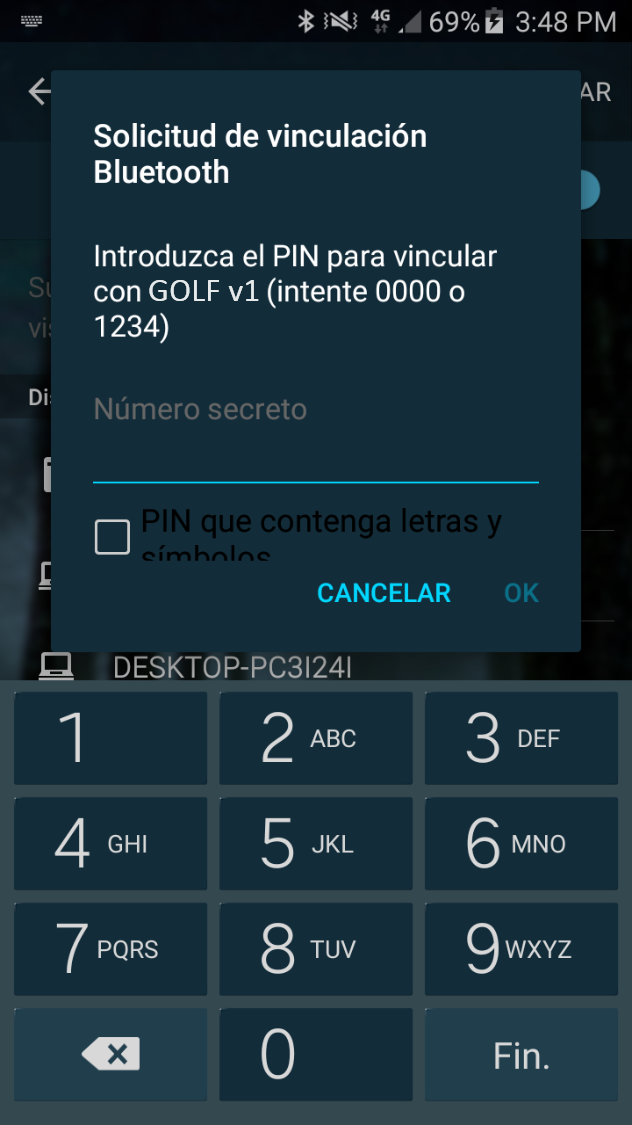
\includegraphics[width=50mm]{metodologia/vinc1.png}}\hspace{5mm}
\subfigure[]{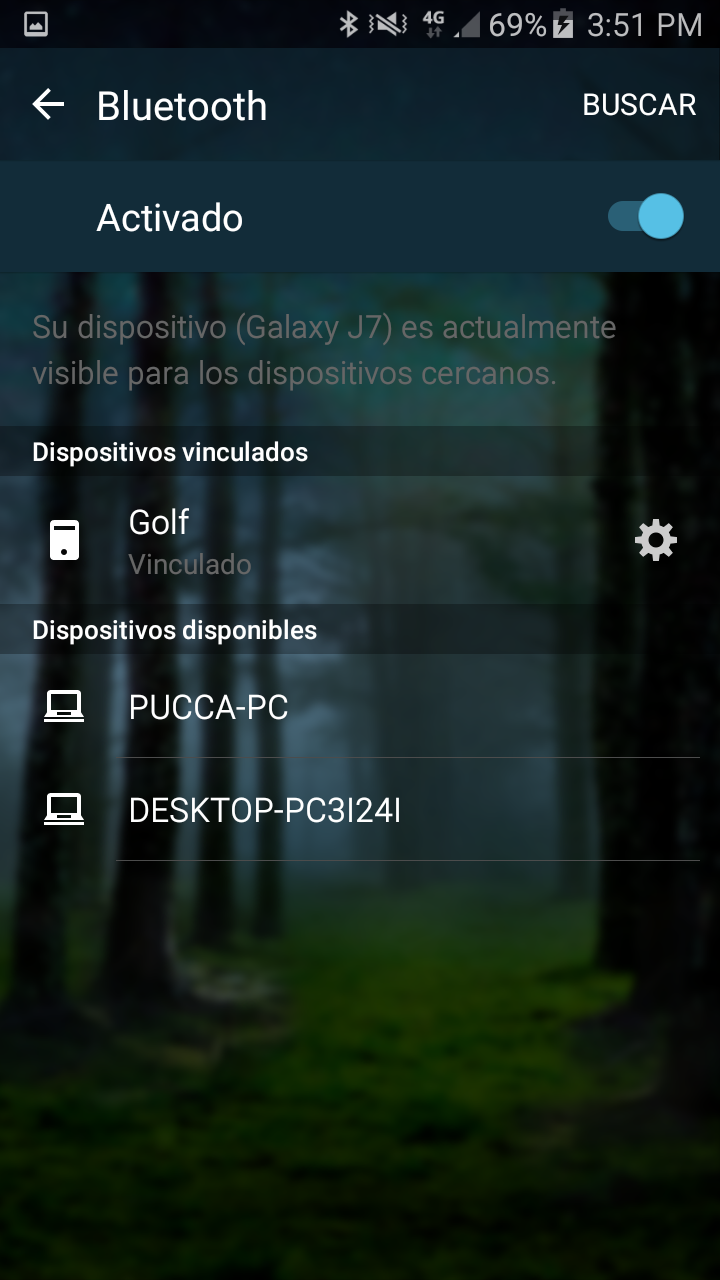
\includegraphics[width=50mm]{metodologia/vinc2.png}}
\caption{Proceso de conexión de bluetooth en el dispositivo móvil.} \label{vinc}
\end{figure}

Una vez finalizado este proceso, la comunicación se realiza con la tarjeta electrónica mediante la aplicación móvil.

\subsection{TARJETA ELECTRÓNICA}

La tarjeta electrónica que se utilizó fue Arduino utilizando el microcontrolador ATMega 3282P, esta se conecta por medio del bluetooth hacia el celular para recibir las variables enviadas.\\



\subsection{CIRCUITO DE POTENCIA}

El circuito de potencia que se elaboró se repite N veces según sean las señales enviadas por parte de la tarjeta electrónica. Este circuito se encarga de recibir la señal de la tarjeta electrónica y activar o desactivar un relevador. Este relevador a su vez permite o denegar el acceso de la señal \textit{low} y así accionar o detener el actuador. El circuito esta conformado por la señal que accede desde la tarjeta electrónica, un capacitor, un transistor y una resistencia armados tal como se muestra en la Figura \ref{circuito_potencia}.  \\

%
%\begin{figure}[H]
%\vspace{0.2cm}
%\centering
%
\includegraphics[width=0.8\textwidth]{metodologia/nodisponible.jpg}
%\caption{circuito de potencia hechizo}
%\label{circuito_potencia}
%\end{figure}

\subsection{ACTUADORES Y SENSORES}

   
\paragraph{Sensor de gas MQ-135}
 (ver Figura \ref{sensor}) sirve para medir el óxido de nitrógeno entre otras cosas, este se coloca dentro del vehículo para medir las emisiones que salen referente al óxido de nitrógeno.\\

%
\begin{figure}[H]
%\vspace{0.2cm}
\centering
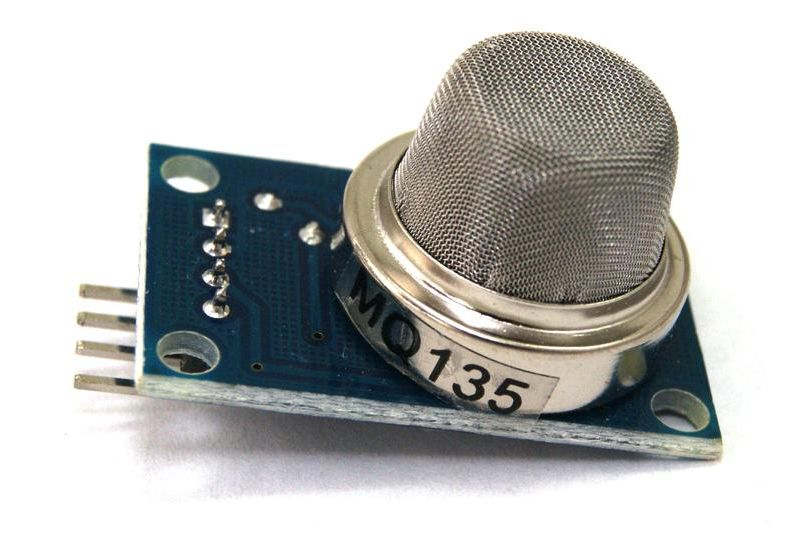
\includegraphics[width=0.5\textwidth]{metodologia/fig_sensor.jpg}
\caption{Conexión del sensor y la tarjeta programable. }
\label{sensor}
\end{figure}
%

La tarjeta del sensor cuenta con dos salidas de datos, una digital (DO) y otra analógica (AO) (ver Figura \ref{descripcion_sensor}). La salida digital manda una señal en estado alto cuando el sensor llega a un nivel deseado, el cual puede ser ajustado por medio del potenciómetro. La salida analógica va aumentado el valor del voltaje en proporción al nivel de gas que se detecta.\\

%
\begin{figure}[H]
%\vspace{0.2cm}
\centering
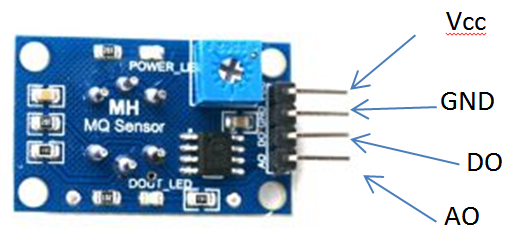
\includegraphics[width=0.5\textwidth]{metodologia/gas_4.png}
\caption{Descripción de las salidas del sensor. }
\label{descripcion_sensor}
\end{figure}
%

Este sensor se conecta directamente a la tarjeta programable, la conexión se muestra en la Figura \ref{conexion_sensor}, para obtener los datos en partes por millón (ppm) es necesario hacer la conversión con el programa que se encuentra en el anexo 1.
%
\begin{figure}[H]
%\vspace{0.2cm}
\centering
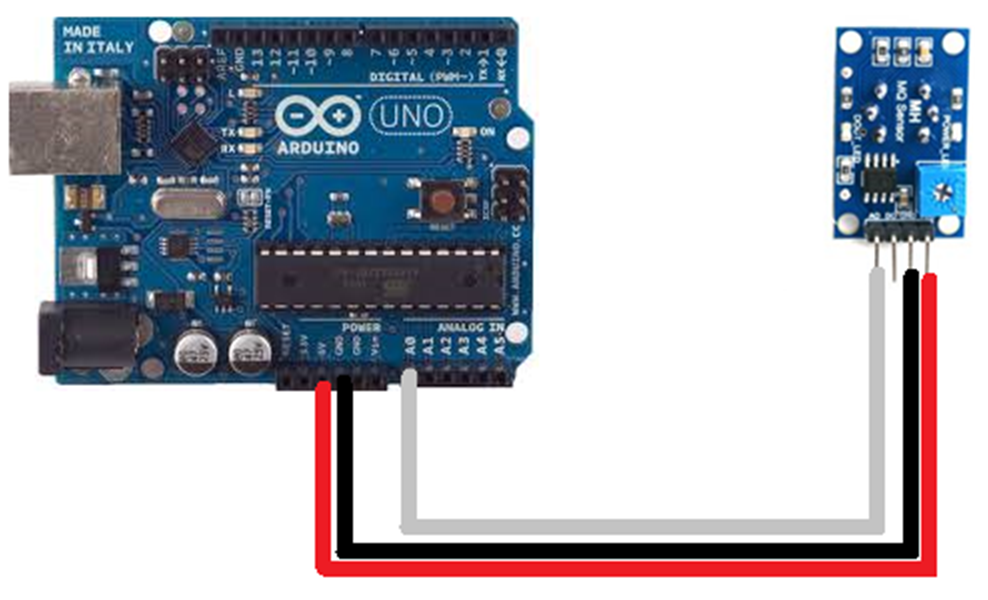
\includegraphics[width=0.5\textwidth]{metodologia/gas_5.png}
\caption{Conexión del sensor y la tarjeta programable. }
\label{conexion_sensor}
\end{figure}
%

la Configuración del puerto serial sirve para cargar el programa e ingresar al monitor serial que ofrece el Arduino es necesario asegurarse que el puerto COM sea el correcto.  Para ello tenemos que acceder a “Administrador de dispositivos” (ver Figura \ref{conf_puerto} desde la PC y verificar que el COM que nos muestra sea el mismo que marca el \textit{software} de Arduino.

\begin{figure}[H]
%\vspace{0.2cm}
\centering
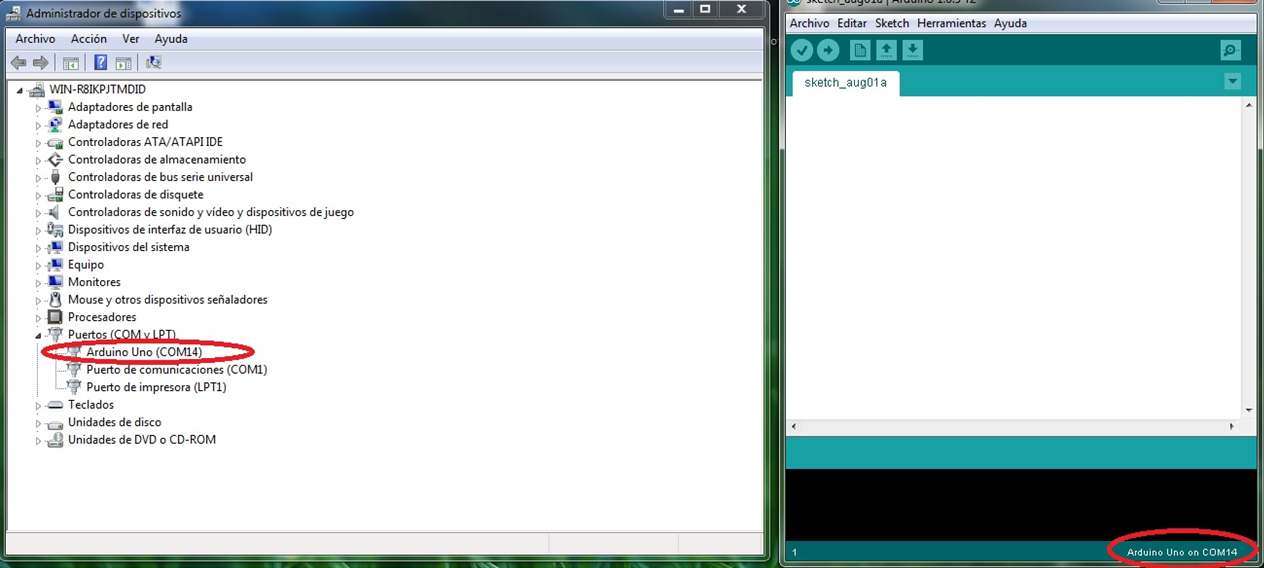
\includegraphics[width=0.5\textwidth]{metodologia/gas_6.png}
\caption{Configurando el puerto serial. }
\label{conf_puerto}
\end{figure}
%

En caso de que no coincida el puerto COM entre el “Administrador de dispositivos” y el marcado en el \textit{software} podemos cambiarlo en la barra de herramientas (ver Figura \ref{conf_puerto2}).

\begin{figure}[H]
%\vspace{0.2cm}
\centering
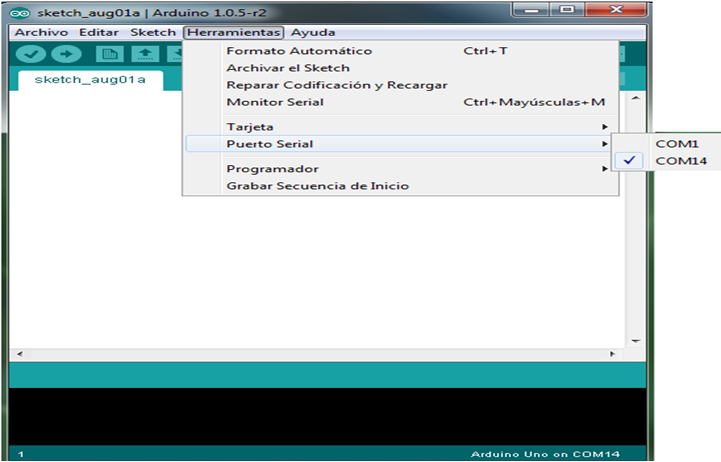
\includegraphics[width=0.5\textwidth]{metodologia/gas_7.png}
\caption{Configurando el puerto desde la barra de herramientas. }
\label{conf_puerto2}
\end{figure}


Una vez que este verificado el puerto serial soló damos clic en la lupa que aparece en la parte superior derecha y automáticamente abre otra ventana que muestra el puerto serial (ver Figura \ref{conf_puerto22}.

\begin{figure}[H]
%\vspace{0.2cm}
\centering
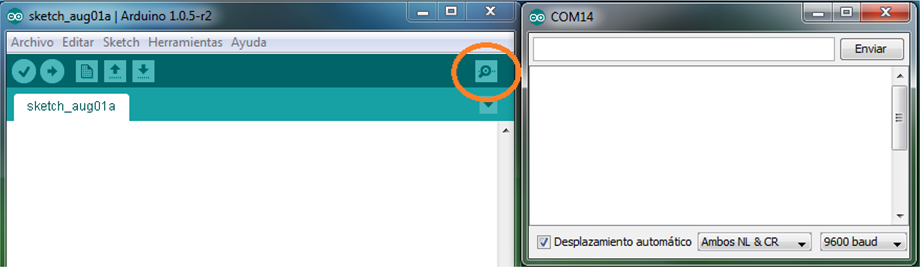
\includegraphics[width=0.5\textwidth]{metodologia/gas_8.png}
\caption{ventana para visualizar la información. }
\label{conf_puerto22}
\end{figure}

\paragraph{Actuador Vidrios Eléctricos} es un mecanismo con un motor electríco incluido de fábrica en algunos vehículos, el auto de prueba maneja un sistema completamente mecánico y a través de una manija eleva o bajar el vidrio.\\

Los pasos que se desarrollaron para automatizar este actuador fueron los siguientes.\\

\begin{enumerate}
\item verificar que las gomas estuvieran en buenas condiciones para evitar que el agua se filtrará dentro de la puerta.\\
\item implementar el motor del elevador de vidrio al sistema mecánico, en esta parse se tuvo la necesidad de adaptar el motor con el sistema de elevación, generando unas ranuras para incluir pernos y así evitar que la fuerza del motor destruyera el sistema de elevación.\\
\item instalar y probar directamente en el acumulador tal cual se muestra en la Figura \ref{subirvidrio}, se implementó un control manual para manipular la actividad de subir y bajar el vidrio. Los diagramas que se ocuparón para el control manual se muestran en la Figura \ref{control_manual}.

\end{enumerate}





\begin{figure}[H]
%\vspace{0.2cm}
\centering
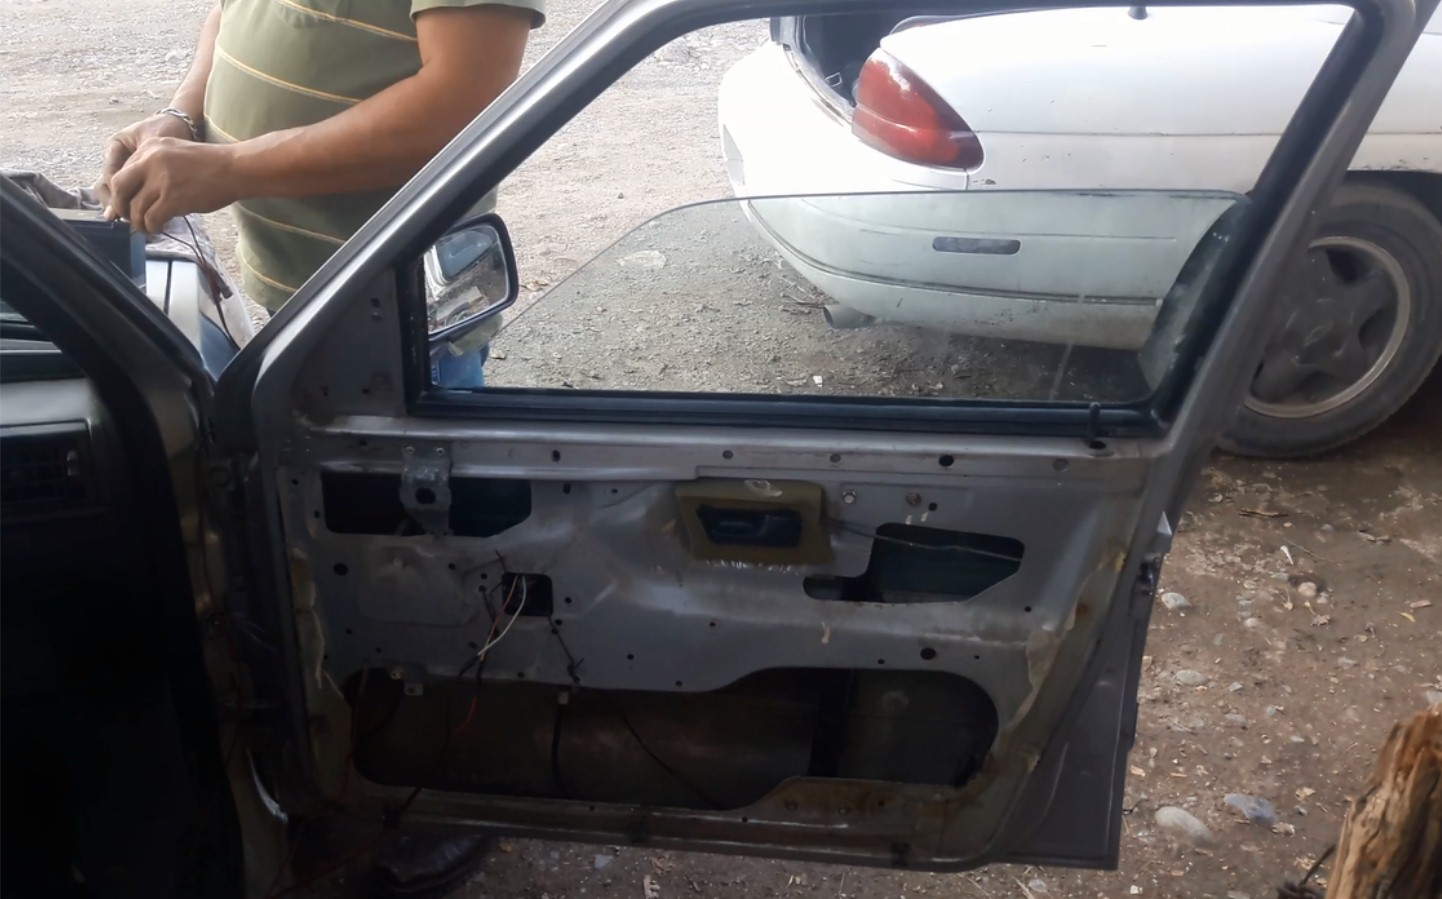
\includegraphics[width=0.7\textwidth]{metodologia/subirvidrio.jpg}
\caption{Instalación del motor en la puerta}
\label{subirvidrio}
\end{figure}

\begin{figure}[H]
%\vspace{0.2cm}
\centering
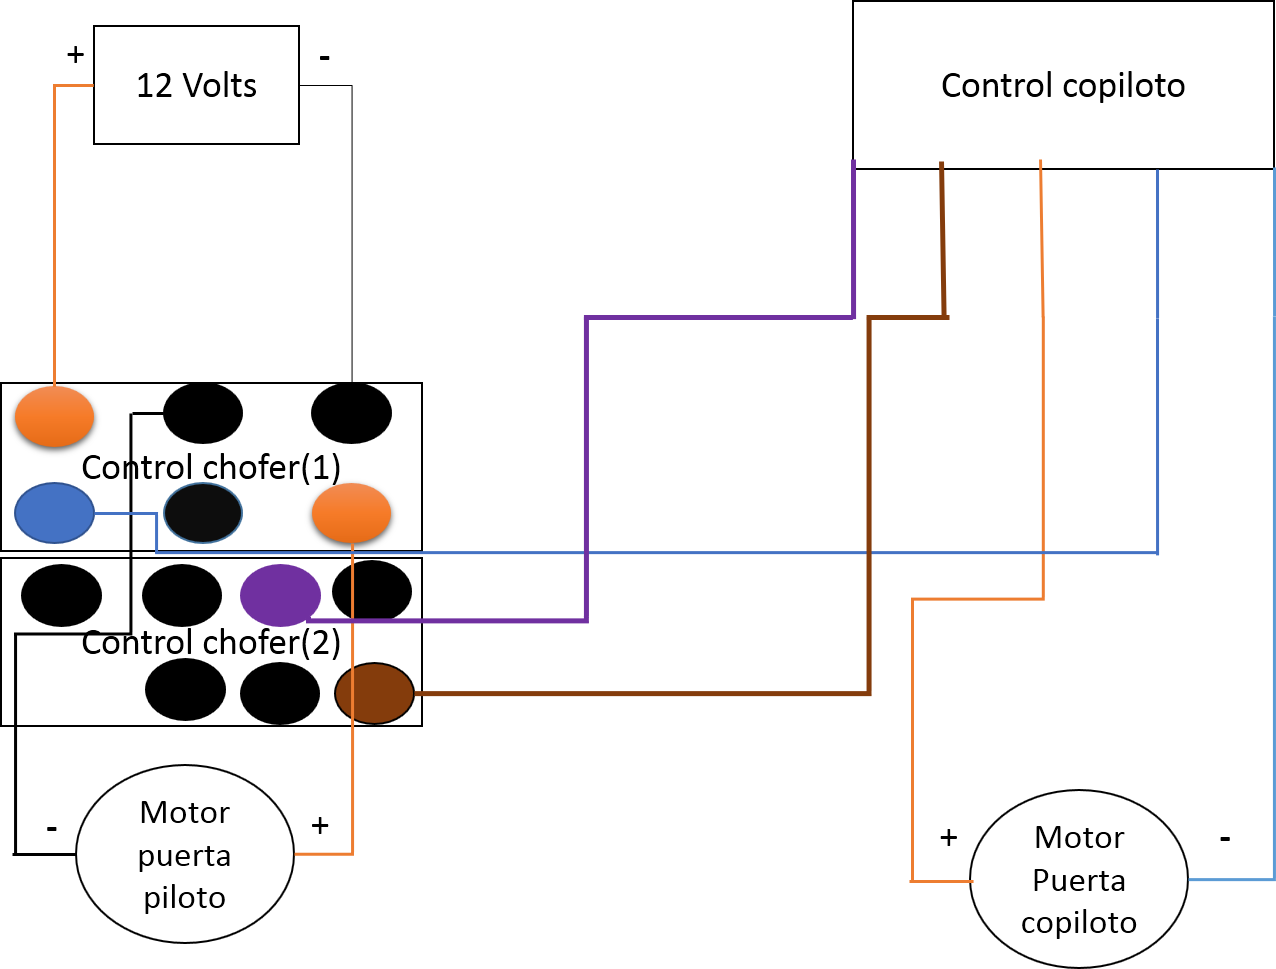
\includegraphics[width=0.7\textwidth]{metodologia/diagramacontrol.png}
\caption{Configuración del control Manual}
\label{control_manual}
\end{figure}

Al final se realizó un circuito generando un puente H para subir y bajar el vidrio con el dispositivo móvil tal cual se muestra en la Figura \ref{circuito_android}, evitando que las señales colisionen entre el control manual y el dispositivo móvil.

%
\begin{figure}[H]
%\vspace{0.2cm}
\centering

\includegraphics[width=0.8\textwidth]{metodologia/nodisponible.jpg}
\caption{XXXX}
\label{circuito_android}
\end{figure}


\paragraph{Actuador Seguros de Puertas}
es un sistema que se le adapta al vehículo para que la puerta no se pueda abrir, evitando accidentes cuando el vehículo se encuentre en movimiento,principalmente.\\

Lo primero que se realizó en esta actividad fue incorporar los seguros e instalarlos dentro de las puertas tal cual se muestra en la Figura \ref{seguros}.
%%
%\begin{figure}[H]
%\vspace{0.2cm}
%\centering
%\includegraphics[width=0.8\textwidth]{metodologia/nodisponible.jpg}
%\caption{XXXX}
%\label{seguros}
%\end{figure}

Una vez instalados se probaron directamente con la batería de vehículo, y se realizó un circuito generando un puente H para subir y bajar el seguro con el dispositivo móvil tal cual se muestra en la Figura\ref{abrir_cerrar_seguros}.
%
%\begin{figure}[H]
%\vspace{0.2cm}
%\centering
%\includegraphics[width=0.8\textwidth]{metodologia/nodisponible.jpg}
%\caption{XXXX}
%\label{abrir_cerrar_seguros}
%\end{figure}


\paragraph{Sistema de Ignición y Marcha}




\paragraph{Actuador Luces Interiores y Exteriores}
un sistema de iluminación interno, normalmente aparece cuando abrimos una puerta o mediante un botón de iluminación. Un sistema de iluminación externo es cuando accionamos un boton para que las luces delanteras se iluminen. 

Lo primero que hicimos fue realizar la estructura y se visualizó la forma de encender mediante el dispositivo móvil las luces, tanto interiores como exteriores.

Luego se realizo el circuito electríco tal cual se muestra en la Figura \ref{luces}, tanto el sistema interno como el externo trabajan de la mismo forma.
%
%\begin{figure}[H]
%\vspace{0.2cm}
%\centering
%\includegraphics[width=0.8\textwidth]{metodologia/nodisponible.jpg}
%\caption{XXXX}
%\label{luces}
%\end{figure}


\paragraph{Actuador Cajuela}
la cajuela es un apartado que tiene el vehículo que permite introducir objetos en él.
para que la cajuela se habrá de manera automática mediante el dispositivo móvil depende de dos actividades, el abrir la cerradura y el levantamiento de la cajuela.
para el abrir la cerradura debe de existir un motor que jale la varilla que hace la función de abrir la cerradura, por la cuestión del levantamiento de la cajuela se cambiaron los pistones, los cuales una vez abierta la cerradura hacen su función de manera inmediata.
